% TU Delft beamer template
% Author: Erwin Walraven (initial version was created by Maarten Abbink)
% Delft Universiy of Technology

\documentclass{beamer}
\usepackage{amsmath}
\usepackage{amsfonts}
\usepackage{amsthm}
\usepackage{mathtools}
\usepackage[english]{babel}
\usepackage{calc}
\usepackage[absolute,overlay]{textpos}
\usepackage{graphicx}
\usepackage{subfig}
\usepackage{comment}
%\usepackage{tikz}
\usepackage{wasysym}
\usepackage{gensymb}
\usepackage{amssymb}
\usepackage{nccmath}
\usepackage{empheq}
\usepackage{xcolor}
\usepackage{relsize}
%\usepackage{apalike}


\newcommand*\widefbox[1]{\fbox{\hspace{1em}#1\hspace{1em}}}
%\useoutertheme{miniframes}

%\usefonttheme[onlymath]{serif}



\setbeamertemplate{navigation symbols}{} % remove navigation symbols
\mode<presentation>{\usetheme{tud}}


%\ExecuteBibliographyOptions{parentracker=false}



% BIB SETTINGS
\usepackage[backend=bibtex,firstinits=true,maxnames=30,maxcitenames=20,url=false,style=authoryear]{biblatex}
%authoryear
\bibliography{MyBib}
%\setcitestyle{square}
\setlength\bibitemsep{0.3cm} % space between entries in the reference list
\renewcommand{\bibfont}{\normalfont\scriptsize}
\setbeamerfont{footnote}{size=\tiny}
\makeatletter
%\renewcommand{\cite}[1]{\footnote<.->[frame][{\fullcite{#1}}]}
%\renewcommand{\cite}[1]{$[$\cite{#1}$]$}


% Insert frame before each subsection (requires 2 latex runs)
\AtBeginSection {
	\begin{frame}<beamer>[noframenumbering] \frametitle{\titleSubsec}
		\tableofcontents[currentsection,currentsubsection]  % Generation of the Table of Contents
	\end{frame}
}

% Define the title of each inserted pre-subsection frame
\newcommand*\titleSubsec{Outline}
% Define the title of the "Table of Contents" frame
\newcommand*\titleTOC{Outline}

\graphicspath{ {./images/} } 

\title[Final MSc Presentation]{Robust output-feedback control of 3D directional drilling systems}
\institute[]{Delft University of Technology, The Netherlands \\ University of Minnesota, USA}
\author{Octavio A. Villarreal Maga\~na \vspace{10pt} \\ \scriptsize Committee:  \\ Prof.Dr.Ir. Nathan van de Wouw (TUDelft, supervisor) \\ \vspace{1.5pt} \hspace{-11pt}Prof.Dr.Ir. Emmanuel Detournay (UMN, supervisor) \\ \vspace{-2.5pt} \hspace{-74pt}Dr.Ir. Manuel Mazo Jr. (TUDelft)}
\date{July 12, 2016}

\begin{document}
{
\setbeamertemplate{footline}{\usebeamertemplate*{minimal footline}}
\frame{\titlepage}
\begin{frame}\frametitle{\titleTOC}
	\tableofcontents
\end{frame}
}

{\setbeamertemplate{footline}{\usebeamertemplate*{minimal footline}}
}

\section{General description of directional drilling systems}

\begin{frame}{Applications of directional drilling}	
	\begin{columns}
	\hspace{0.9cm}\begin{column}{0.4\textwidth}
	\begin{figure}[t]
		\centering
		\begin{minipage}[t]{1\textwidth}
			\centering
			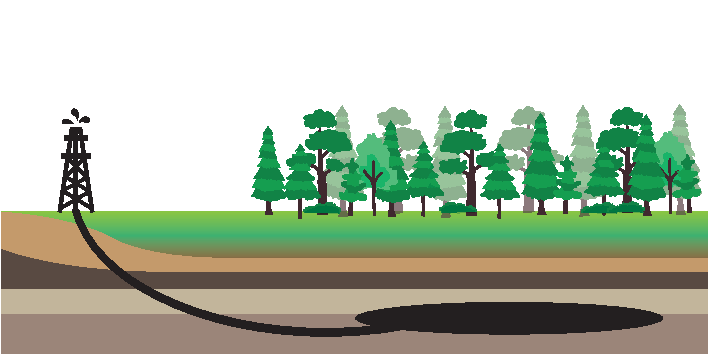
\includegraphics[width=1\linewidth]{images/appdd1.pdf}\\
		\end{minipage}%\\
		\\\begin{minipage}[t]{1\textwidth}
			\centering
			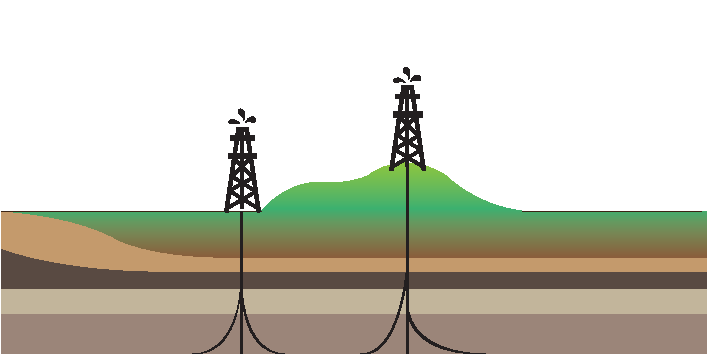
\includegraphics[width=1\linewidth]{images/appdd2.pdf}\\
		\end{minipage}
		\begin{minipage}[t]{1\textwidth}
			\centering
			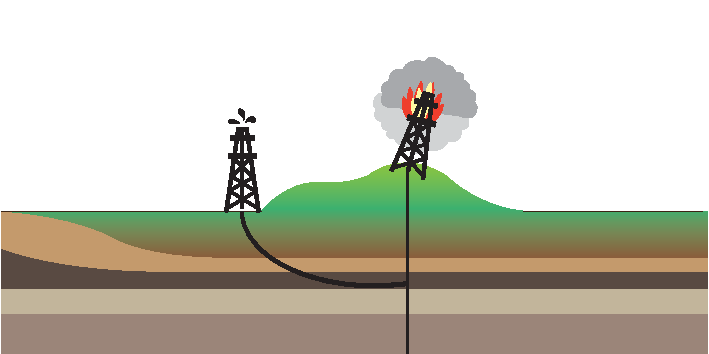
\includegraphics[width=1\linewidth]{images/appdd3.pdf}\\
		\end{minipage}
	\end{figure}
	\end{column}
	\begin{column}{0.6\textwidth}\setlength{\leftmargini}{20pt}
		\begin{itemize}\setlength\itemsep{2.5em}
			\item Extract oil, mineral and thermal energy resources
			\item Reach targets that need complex geometries such as:
				\begin{itemize}\setlength\itemsep{1em}
					\item Under a city or an ecosystem
					\item Far from the drill rig
					\item Relief for hazardous situations
				\end{itemize}
		\end{itemize}
	\end{column}
	\end{columns}
\end{frame}

\begin{frame}\frametitle{General description of the system}
	\begin{columns}
	\hspace{1cm}	\begin{column}{0.6\textwidth}
		\begin{figure}[ht]\centering
				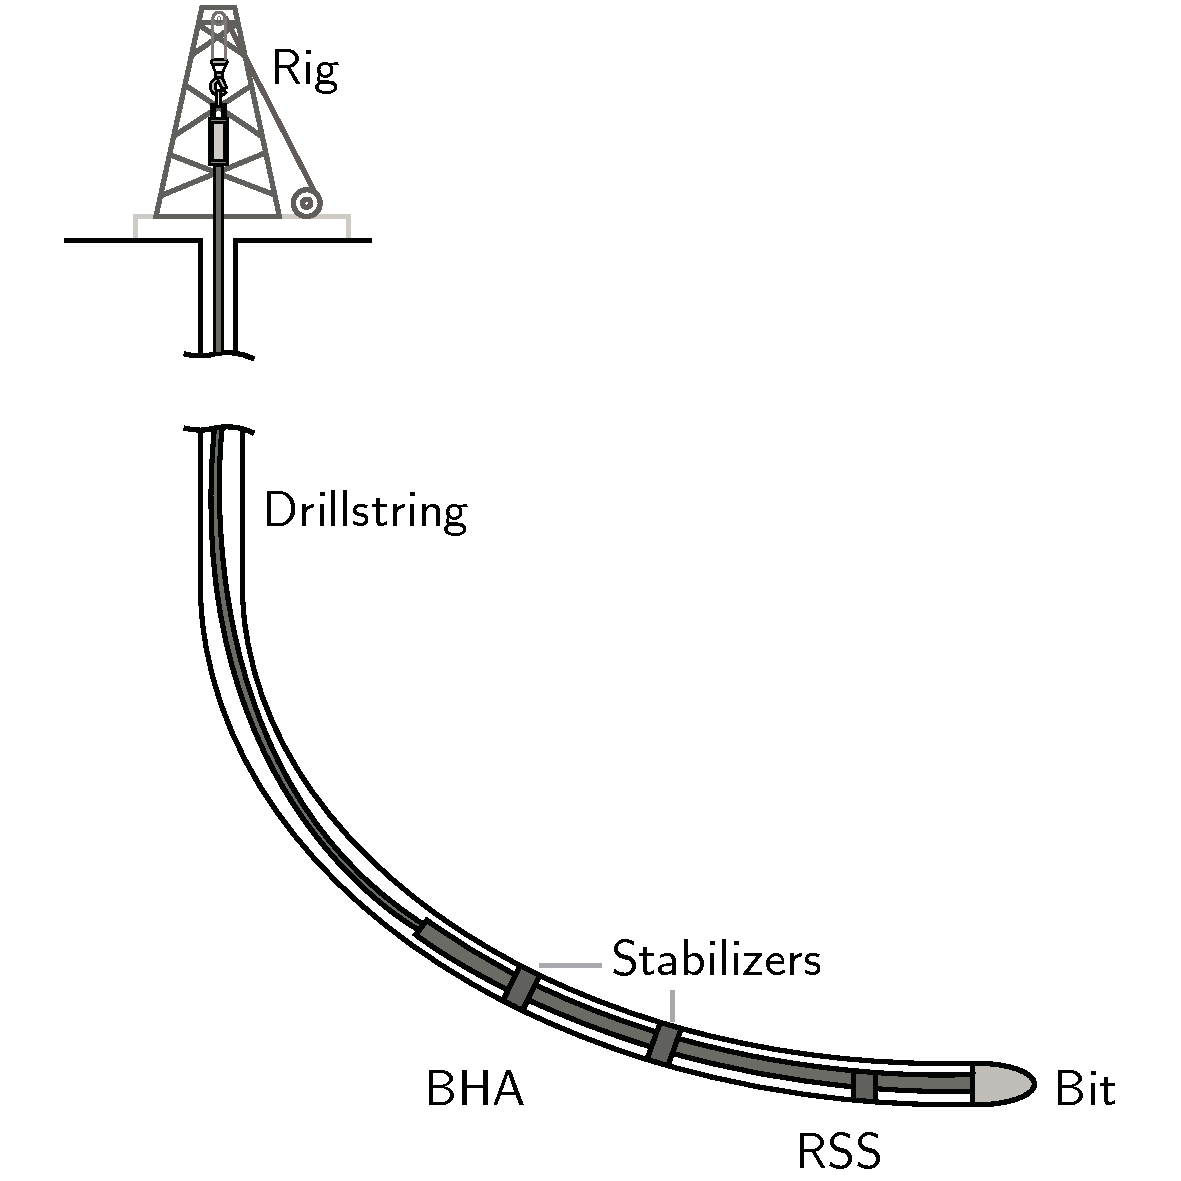
\includegraphics[width=1\textwidth]{images/drillingsystem.pdf}
			\end{figure}
		\end{column}
		\begin{column}{0.4\textwidth}
			\centering
			Rotary Steerable System
			\vspace{-10pt}	
			\begin{figure}[ht]
				\begin{minipage}[t]{1\textwidth}
				\hspace{0.5cm}	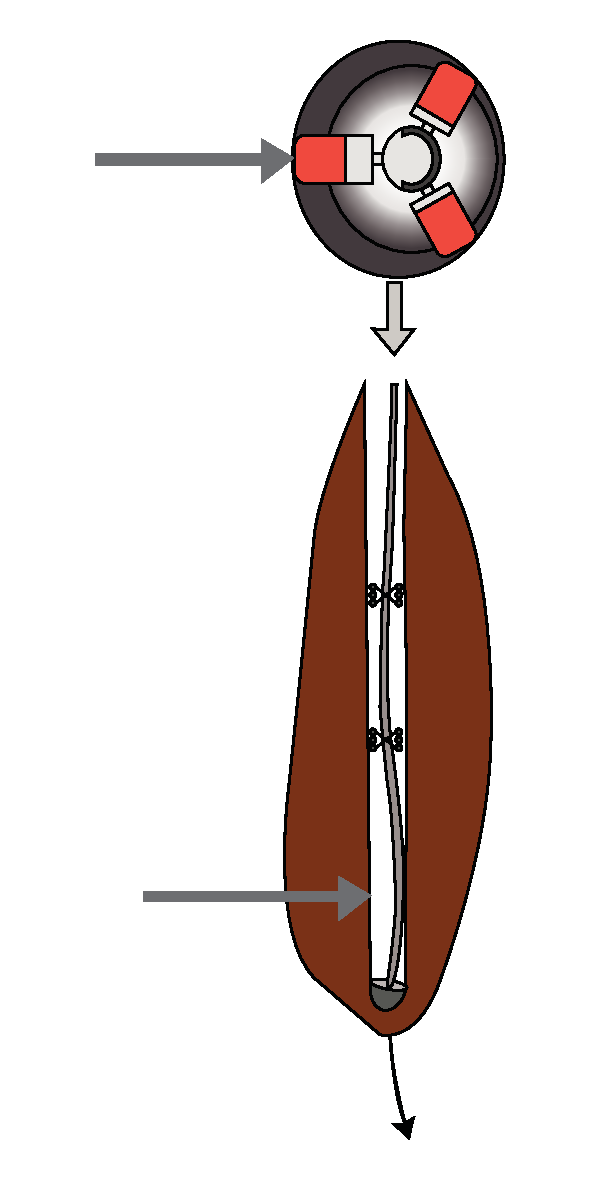
\includegraphics[width=0.5\textwidth]{images/RSS.pdf}
				\end{minipage}
				\begin{minipage}[b]{1\textwidth}
			\hspace{1.1cm} 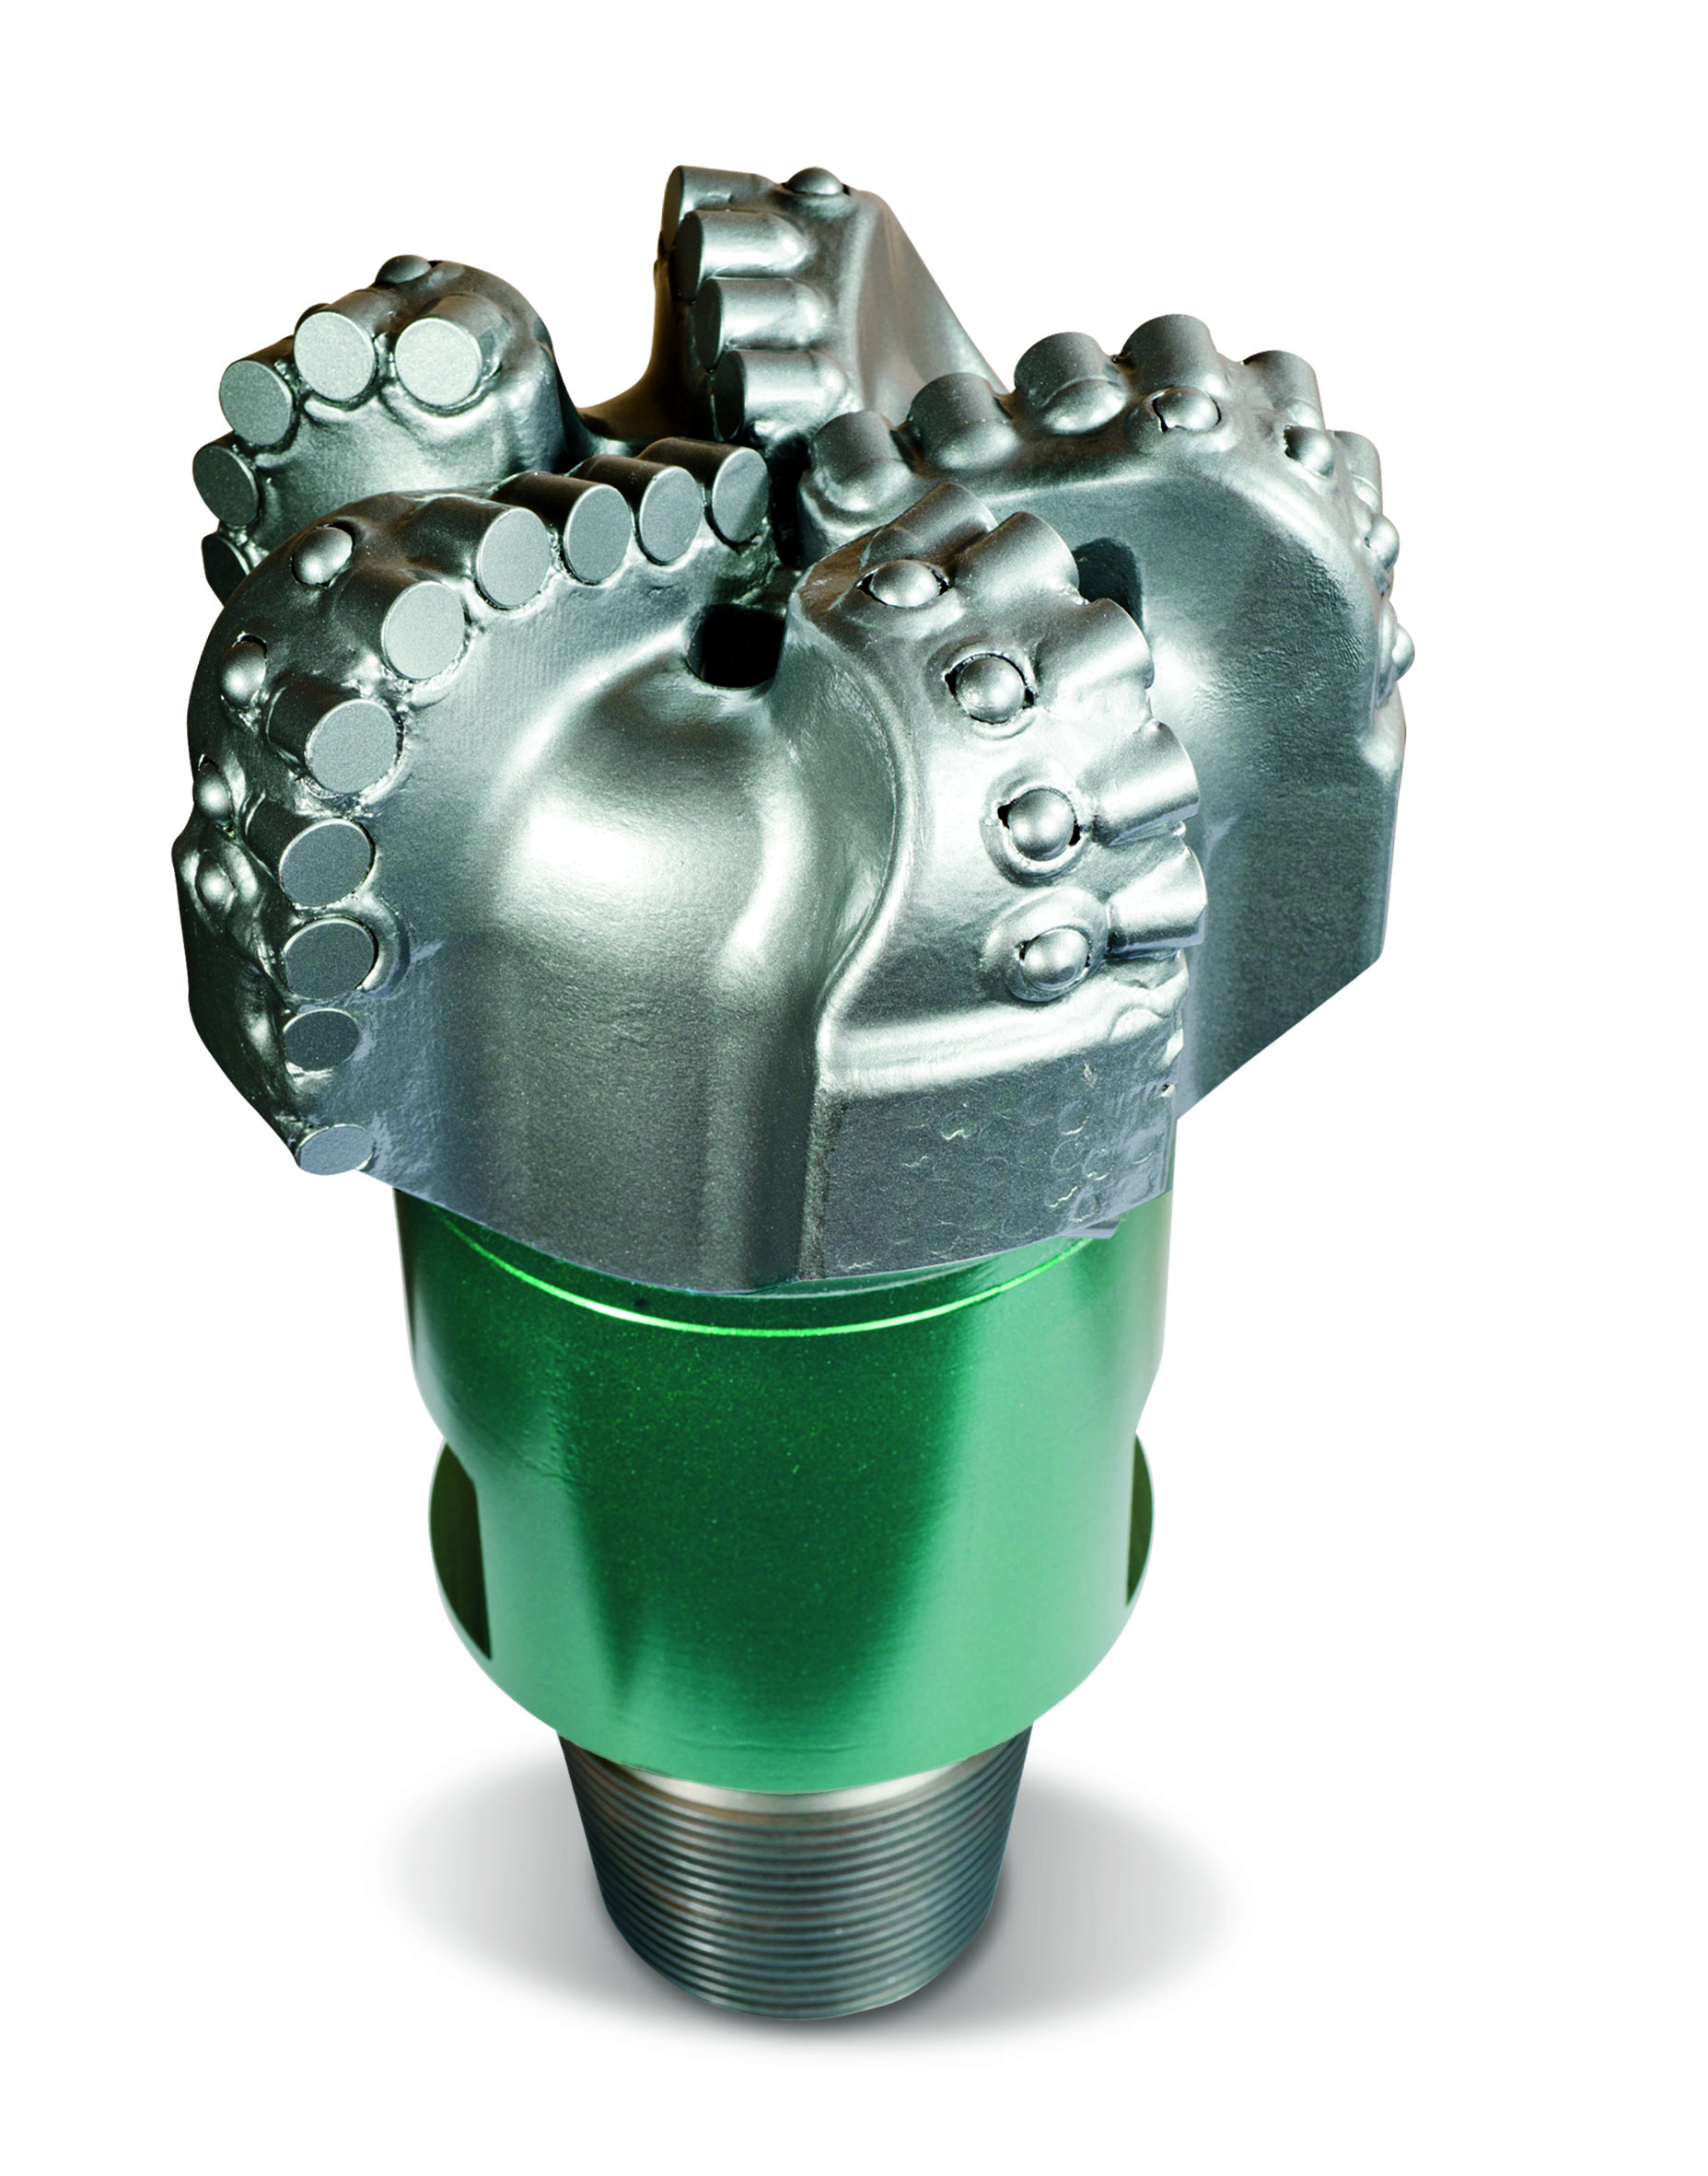
\includegraphics[width=0.4\textwidth]{images/PDC-bit.pdf}
			\end{minipage}
			\end{figure}			
		\end{column}
	\end{columns}
\end{frame}



\begin{frame}{Context and challenges}
		\begin{columns}[T]
		\hspace{1cm}	\begin{column}{0.5\textwidth}\setlength{\leftmargini}{0pt}
				\vspace{1cm}
				\begin{figure}[ht]\centering
					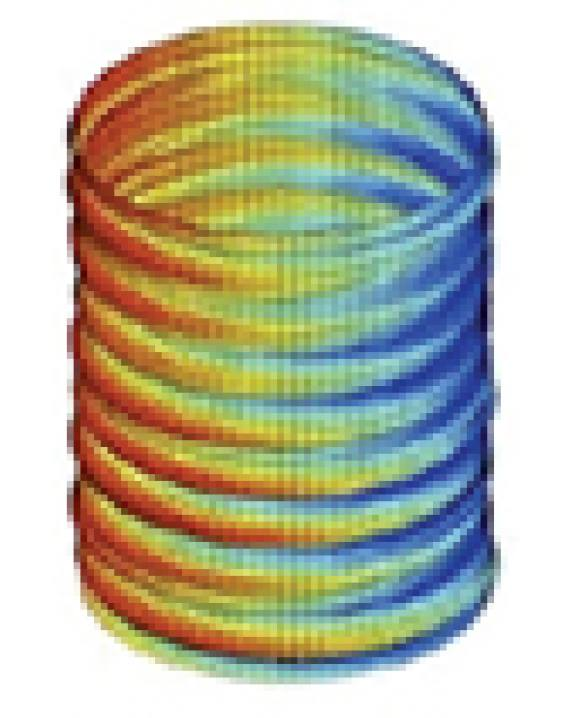
\includegraphics[width=0.5\textwidth]{images/Spiraling.png}
				\end{figure}
			\end{column}
			\begin{column}{0.6\textwidth}\setlength{\leftmargini}{0pt}
				\begin{itemize}
					\setlength\itemsep{3.5em}
					\item State-of-practice: Constant RSS force
					\item Negative effects: kinking, rippling and spiraling
					\item Process consequences of negative effects: reduced ROP and accuracy
				\end{itemize}			
			\end{column}
		\end{columns}
\end{frame}

\begin{frame}{Research goal}
	\textbf{\Large Develop a control strategy for a 3D directional drilling system, that allows to drill boreholes with complex geometries.}
\end{frame}

\begin{frame}{Previous works}
	\begin{itemize}\setlength\itemsep{2.5em}
		\item PD model of 3D directional drilling systems $[$\cite{Perneder2013}$]$
		\item Model-based decoupled control of a 3D directional drilling system $[$\cite{Monsieurs2015}$]$
		\begin{itemize}\setlength\itemsep{1em}
			\item State-feedback controller
			\item Relies on availability of measurements of the states (not possible)
			\item Not "a priori" robustly stable 
		\end{itemize}
	\end{itemize}
\end{frame}

\begin{frame}{Subgoals}
	\begin{itemize}\setlength\itemsep{2.5em}
		\item \textbf{Control strategy that relies only in local measurements (observer design)}
		\item \textbf{Robustness against parametric uncertainty}
	\end{itemize}
\end{frame}

\section{Mathematical model}


\begin{frame}\frametitle{Geometric description}
	\begin{columns}[T]
		\hspace{1cm}\begin{column}{0.5\textwidth}
			\vspace{-20pt}
			\begin{itemize} 
			\item <1|only@1> [] \vspace{3pt}\begin{figure}[ht]\centering
									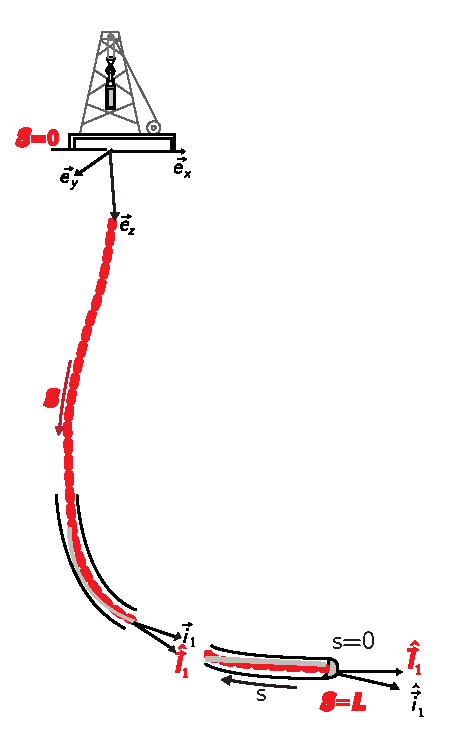
\includegraphics[width=1\textwidth]{images/geodesca.pdf}
								\end{figure}
			\item <2|only@2> [] \vspace{3pt}\begin{figure}[ht]\centering
				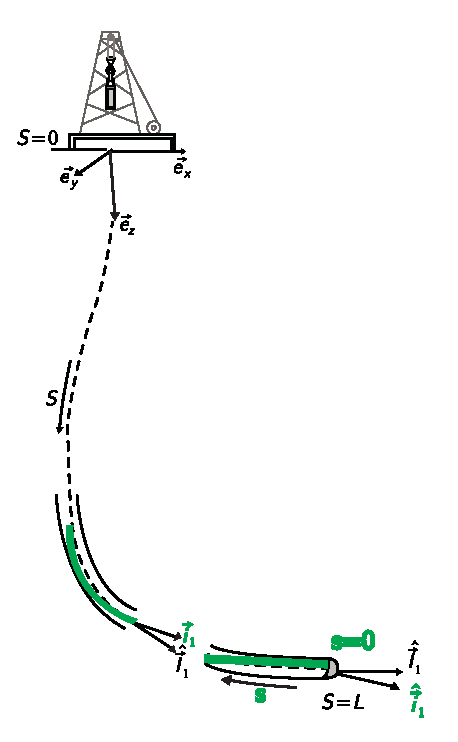
\includegraphics[width=1\textwidth]{images/geodescb.pdf}
			\end{figure}
			\end{itemize}
		\end{column}
		\begin{column}{0.5\textwidth}
			\begin{itemize}
				\item <1|only@1> [] \begin{figure}\centering
					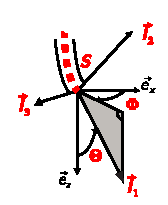
\includegraphics[width=0.9\textwidth]{images/geodesc1a.pdf}
				\end{figure}
				$\Theta (L)$ and $\Phi (L)$: Describe borehole evolution
				\item <2|only@2> [] \begin{figure}\centering
					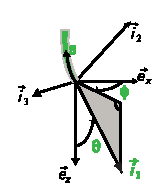
\includegraphics[width=0.9\textwidth]{images/geodesc2b.pdf}
				\end{figure}
				Only measurements of BHA
			\end{itemize}
		\end{column}
	\end{columns}
\end{frame}

\begin{frame}{RSS actuator}
	\begin{columns}[T]
			\begin{column}{0.5\textwidth}
			\hspace{2cm}	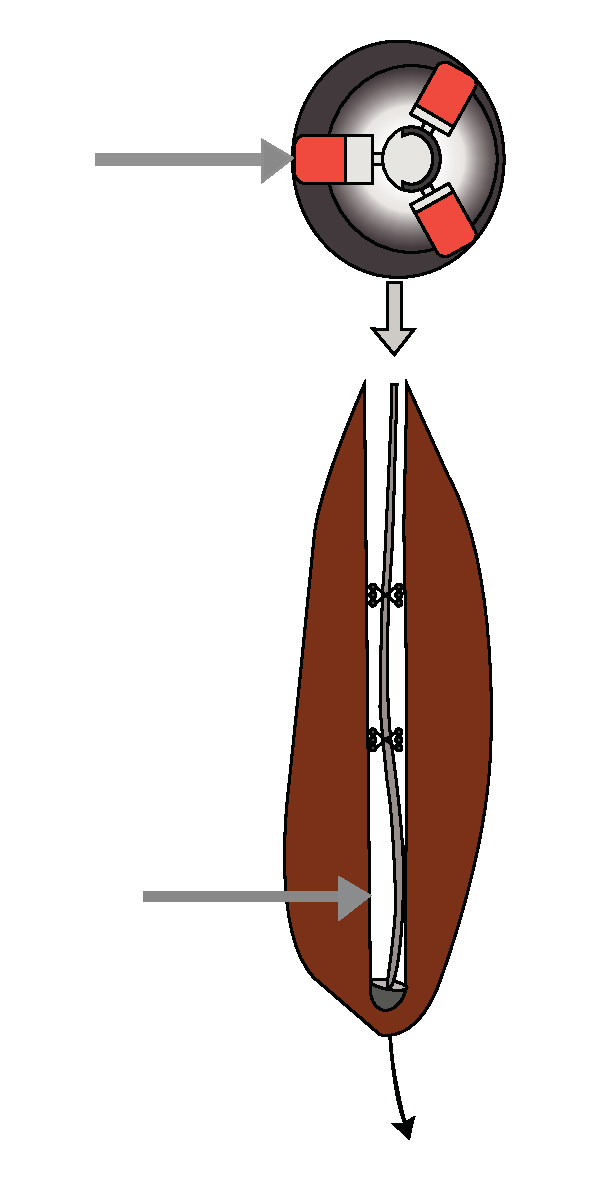
\includegraphics[width=0.5\textwidth]{images/RSSForce0.pdf}
			\end{column}
			\begin{column}{0.5\textwidth}
					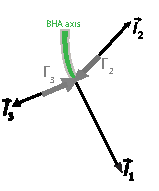
\includegraphics[width=0.9\textwidth]{images/RSSForce.pdf}				
			\end{column}
		\end{columns}
\end{frame}

\begin{frame}{Elements of the model}
	\begin{figure}[ht]\centering
		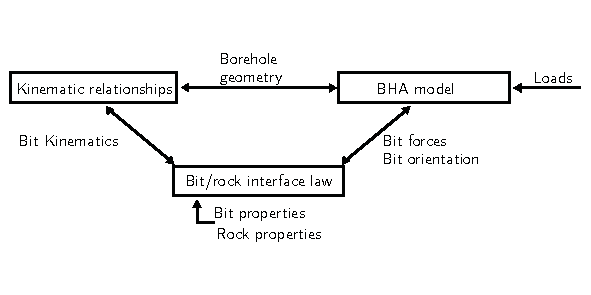
\includegraphics[width=1\textwidth]{images/modelinteraction.pdf}
	\end{figure}\vspace{-20pt}
	\begin{itemize}\setlength\itemsep{0.5em}
			\item Nonlinear delay differential equations (Fit BHA in already drilled borehole)
			\item Function of length $\xi$
		\end{itemize}
\end{frame}


\begin{frame}{System parameters}
 \begin{columns}[T]
		\begin{column}{0.45\textwidth}
			\begin{figure}[ht]\centering
				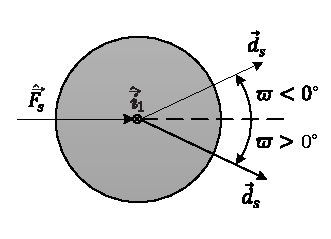
\includegraphics[width=1\textwidth]{images/Drawing_bitwalk.pdf}
			\end{figure}
			\begin{figure}[ht]\centering
			\vspace{-1cm}	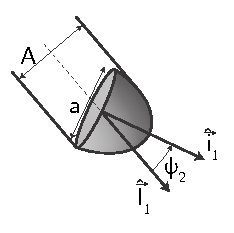
\includegraphics[width=0.8\textwidth]{images/Overgauge.pdf}
			\end{figure}
		\end{column}
		\begin{column}{0.5\textwidth}\setlength{\leftmargini}{0pt}
			\vspace{1cm}\begin{itemize}\setlength\itemsep{2.5em}
				\item Constant
						\begin{itemize}\setlength\itemsep{1em}
							\item Angular steering resistance $\eta$
							\item Lateral steering resistance $\chi$
						\end{itemize}
				\item Uncertain
				\begin{itemize} \setlength\itemsep{1em}
					\item Active weight on bit $\Pi$ (Hookload, drag forces, bit sharpness).
				\item Bit walk angle $\varpi$ (bit orientation, overgauging).
					\end{itemize}
			\end{itemize}
		\end{column}
	\end{columns}
\end{frame}

\begin{frame}{Borehole evolution equations}
		\begin{align*}
		\Theta'(\xi) &= f_\Theta (\Theta,\Phi,\Gamma_2,\Gamma_3,\varpi,\Pi) \\
		\Phi'(\xi) &= f_\Phi (\Theta,\Phi,\Gamma_2,\Gamma_3,\varpi,\Pi)
		\end{align*}
		Non-neutral vs neutral bit walk tendency:
		\begin{figure}[ht]\centering
				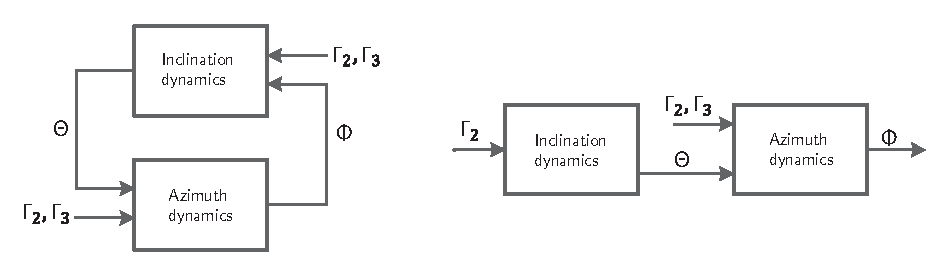
\includegraphics[width=1\textwidth]{images/ModelComparison.pdf}
		\end{figure}
		\begin{columns}[T]
				\begin{column}{0.47\textwidth}\centering
					\LARGE$\varpi \ne 0$
				\end{column}
				\begin{column}{0.47\textwidth}\centering
					\LARGE$\varpi = 0$
				\end{column}
		\end{columns}
\end{frame}


\begin{frame}{Neutral bit walk evolution equations}\setlength{\leftmargini}{0pt}


	\begin{itemize}
		\item <1|only@1> [] \vspace{-1.0cm} Two stabilizers case: \footnotesize
		\begin{equation}
		\begin{aligned}
		\chi \Pi \Theta ' =  &- \mathcal{M}_b(\Theta-\langle\Theta \rangle_1)-\frac{{{\mathcal{M}_b}{\mathcal{F}_1} + {\mathcal{M}_1}\left( {\eta \Pi  - {\mathcal{F}_b}} \right)}}{{\eta \Pi }}\left( {{\langle{\Theta} \rangle_1} - {\langle{\Theta} \rangle_{2}}} \right)
		\\
		&+\frac{\chi }{\eta }{\mathcal{F}_b}\left( {{\Theta} - {{\Theta}_1}} \right)
		- \frac{\chi }{\eta }{\mathcal{F}_1}\left( {{{{{\Theta}} - {{\Theta}_1}}} - \frac{{{{\Theta}_1} - {{\Theta}_{2}}}}{{{\varkappa _{2}}}}} \right)
		\\
		&- \frac{{{\mathcal{M}_b}{\mathcal{F}_r} + (\eta \Pi  - {\mathcal{F}_b}){\mathcal{M}_r}}}{{\eta \Pi }}{\Gamma _{\Theta}} - \frac{\chi }{\eta }{\mathcal{F}_r}\Gamma_{\!\Theta}' + W
		\\
		\chi \Pi \Phi ' =  &- {\mathcal{M}_b}\left( {\Phi  - {\langle{\Phi} \rangle_1}} \right)-\frac{{{\mathcal{M}_b}{\mathcal{F}_1} + {\mathcal{M}_1}\left( {\eta \Pi  - {\mathcal{F}_b}} \right)}}{{\eta \Pi }}\left( {{\langle{\Phi} \rangle_1} - {\langle{\Phi} \rangle_{2}}} \right)
		\\
		&+\frac{\chi }{\eta }{\mathcal{F}_b}\left( {{\Phi} - {{\Phi}_1}} \right)
		- \frac{\chi }{\eta }{\mathcal{F}_1}\left( {{{{{\Phi}} - {{\Phi}_1}}} - \frac{{{{\Phi}_1} - {{\Phi}_{2}}}}{{{\varkappa _{2}}}}} \right)
		\\
		&+ \left( {\frac{\chi }{\eta }\frac{{{\mathcal{F}_r}\Theta '\cos \Theta }}{{{{\left( {\sin \Theta } \right)}^2}}} - \frac{{{\mathcal{M}_b}{\mathcal{F}_r} + {\mathcal{M}_r}\left( {\eta \Pi  - {\mathcal{F}_b}} \right)}}{{\eta \Pi \sin \Theta }}} \right){\Gamma _{\Phi}} - \frac{\chi }{\eta }\frac{{{\mathcal{F}_r}}}{{\sin \Theta }}\Gamma_{\!\Phi}'
		\end{aligned}
		\nonumber
		\end{equation}
		%
		%
		%
		\item <2|only@2> [] \vspace{-0.4cm} Two stabilizers case: \footnotesize
	\begin{equation}
			\begin{aligned}
			\color{gray}\chi \Pi \Theta ' =  &\color{gray}- \color{black}\mathcal{M}_b\color{gray}(\Theta-\langle\Theta \rangle_1)-\frac{{{\color{black}\mathcal{M}_b\color{gray}}{\color{black}\mathcal{F}_1\color{gray}} + {\color{black}\mathcal{M}_1\color{gray}}\left( {\eta \Pi  - {\color{black}\mathcal{F}_b\color{gray}}} \right)}}{{\eta \Pi }}\left( {{\langle{\Theta} \rangle_1} - {\langle{\Theta} \rangle_{2}}} \right)
			\\
			&\color{gray}+\frac{\chi }{\eta }{\color{black}\mathcal{F}_b\color{gray}}\left( {{\Theta} - {{\Theta}_1}} \right)
			- \frac{\chi }{\eta }{\color{black}\mathcal{F}_1\color{gray}}\left( {{{{{\Theta}} - {{\Theta}_1}}} - \frac{{{{\Theta}_1} - {{\Theta}_{2}}}}{{{\varkappa _{2}}}}} \right)
			\\
			&\color{gray}- \frac{{{\color{black}\mathcal{M}_b\color{gray}}{\color{black}\mathcal{F}_r\color{gray}} + (\eta \Pi  - {\color{black}\mathcal{F}_b\color{gray}}){\color{black}\mathcal{M}_r\color{gray}}}}{{\eta \Pi }}{\Gamma _{\Theta}} - \frac{\chi }{\eta }{\color{black}\mathcal{F}_r\color{gray}}\Gamma_{\!\Theta}' + W
			\\
			\color{gray}\chi \Pi \Phi ' =  &\color{gray}- {\color{black}\mathcal{M}_b\color{gray}}\left( {\Phi  - {\langle{\Phi} \rangle_1}} \right)-\frac{{{\color{black}\mathcal{M}_b\color{gray}}{\color{black}\mathcal{F}_1\color{gray}} + {\color{black}\mathcal{M}_1\color{gray}}\left( {\eta \Pi  - {\color{black}\mathcal{F}_b\color{gray}}} \right)}}{{\eta \Pi }}\left( {{\langle{\Phi} \rangle_1} - {\langle{\Phi} \rangle_{2}}} \right)
			\\
			&\color{gray}+\frac{\chi }{\eta }{\color{black}\mathcal{F}_b\color{gray}}\left( {{\Phi} - {{\Phi}_1}} \right)
			- \frac{\chi }{\eta }{\color{black}\mathcal{F}_1\color{gray}}\left( {{{{{\Phi}} - {{\Phi}_1}}} - \frac{{{{\Phi}_1} - {{\Phi}_{2}}}}{{{\varkappa _{2}}}}} \right)
			\\
			&\color{gray}+ \left( {\frac{\chi }{\eta }\frac{{{\color{black}\mathcal{F}_r\color{gray}}\Theta '\cos \Theta }}{{{{\left( {\sin \Theta } \right)}^2}}} - \frac{{{\color{black}\mathcal{M}_b\color{gray}}{\color{black}\mathcal{F}_r\color{gray}} + {\color{black}\mathcal{M}_r\color{gray}}\left( {\eta \Pi  - {\color{black}\mathcal{F}_b\color{gray}}} \right)}}{{\eta \Pi \sin \Theta }}} \right){\Gamma _{\Phi}} - \frac{\chi }{\eta }\frac{{{\color{black}\mathcal{F}_r\color{gray}}}}{{\sin \Theta }}\Gamma_{\!\Phi}'
			\end{aligned}
			\nonumber
			\end{equation}
		\\
		\begin{itemize}\setlength\itemsep{0.5em}
		\item []  	\normalsize \textbf{BHA configuration constant coefficients}
		\end{itemize}
		%
		%
		%
		\item <3|only@3> []  \vspace{0.3cm} Two stabilizers case: \footnotesize
		\begin{equation}
		\begin{aligned}
		\color{gray}\chi \Pi \Theta ' =  &\color{gray}- \mathcal{M}_b(\Theta-\color{black}\langle\Theta \rangle_1\color{gray})-\frac{{{\mathcal{M}_b}{\mathcal{F}_1} + {\mathcal{M}_1}\left( {\eta \Pi  - {\mathcal{F}_b}} \right)}}{{\eta \Pi }}\left( {{\color{black}\langle\Theta \rangle_1\color{gray}} - {\color{black}\langle\Theta \rangle_2\color{gray}}} \right)
		\\
		&\color{gray}+\frac{\chi }{\eta }{\mathcal{F}_b}\left( {{\Theta} - {{\Theta}_1}} \right)
		- \frac{\chi }{\eta }{\mathcal{F}_1}\left( {{{{{\Theta}} - {{\Theta}_1}}} - \frac{{{{\Theta}_1} - {{\Theta}_{2}}}}{{{\varkappa _{2}}}}} \right)
		\\
		&\color{gray}- \frac{{{\mathcal{M}_b}{\mathcal{F}_r} + (\eta \Pi  - {\mathcal{F}_b}){\mathcal{M}_r}}}{{\eta \Pi }}{\Gamma _{\Theta}} - \frac{\chi }{\eta }{\mathcal{F}_r}\Gamma_{\!\Theta}' + W
		\\
		\color{gray}\chi \Pi \Phi ' =  &\color{gray}- {\mathcal{M}_b}\left( {\Phi  - {\color{black}\langle{\Phi} \rangle_1\color{gray}}} \right)-\frac{{{\mathcal{M}_b}{\mathcal{F}_1} + {\mathcal{M}_1}\left( {\eta \Pi  - {\mathcal{F}_b}} \right)}}{{\eta \Pi }}\left( {{\color{black}\langle{\Phi} \rangle_1\color{gray}} - {\color{black}\langle{\Phi} \rangle_2\color{gray}}} \right)
		\\
		&\color{gray}+\frac{\chi }{\eta }{\mathcal{F}_b}\left( {{\Phi} - {{\Phi}_1}} \right)
		- \frac{\chi }{\eta }{\mathcal{F}_1}\left( {{{{{\Phi}} - {{\Phi}_1}}} - \frac{{{{\Phi}_1} - {{\Phi}_{2}}}}{{{\varkappa _{2}}}}} \right)
		\\
		&\color{gray}+ \left( {\frac{\chi }{\eta }\frac{{{\mathcal{F}_r}\Theta '\cos \Theta }}{{{{\left( {\sin \Theta } \right)}^2}}} - \frac{{{\mathcal{M}_b}{\mathcal{F}_r} + {\mathcal{M}_r}\left( {\eta \Pi  - {\mathcal{F}_b}} \right)}}{{\eta \Pi \sin \Theta }}} \right){\Gamma _{\Phi}} - \frac{\chi }{\eta }\frac{{{\mathcal{F}_r}}}{{\sin \Theta }}\Gamma_{\!\Phi}'
		\end{aligned}
		\nonumber
		\end{equation}\\
		 Averages (Distributed delays):
		\begin{align*}
			{{\rm{\langle\Theta\rangle }}_i}:= \frac{1}{\varkappa_i}\int \limits_{\xi_{i}}^{\xi_{i-1}} \Theta(\sigma)d\sigma, \qquad
			{{\rm{\langle\Phi\rangle }}_i}:=\frac{1}{\varkappa_i}\int \limits_{\xi_{i}}^{\xi_{i-1}} \Phi(\sigma)d\sigma
			\label{eq:definitionaveragestates} \\
			\varkappa_i: \text{Length between stabilizers}, \qquad \text{ for } i = 1,2
		\end{align*}
		%
		%
		%
		\item <4|only@4> [] Two stabilizers case: \footnotesize
		\begin{equation}
		\begin{aligned}
		\color{gray}\chi \Pi \Theta ' =  &\color{gray}- \mathcal{M}_b(\Theta-\langle\Theta \rangle_1)-\frac{{{\mathcal{M}_b}{\mathcal{F}_1} + {\mathcal{M}_1}\left( {\eta \Pi  - {\mathcal{F}_b}} \right)}}{{\eta \Pi }}\left( {{\langle{\Theta} \rangle_1} - {\langle{\Theta} \rangle_{2}}} \right)
		\\
		&\color{gray}+\frac{\chi }{\eta }{\mathcal{F}_b}\left( {{\Theta} - {\color{black}{\Theta}_1 \color{gray}}} \right)
		- \frac{\chi }{\eta }{\mathcal{F}_1}\left( {{{{{\Theta}} - {\color{black}{\Theta}_1\color{gray}}}} - \frac{{{\color{black}{\Theta}_1\color{gray}} - \color{black}{{\Theta}_{2}\color{gray}}}}{{{\varkappa _{2}}}}} \right)
		\\
		&\color{gray}- \frac{{{\mathcal{M}_b}{\mathcal{F}_r} + (\eta \Pi  - {\mathcal{F}_b}){\mathcal{M}_r}}}{{\eta \Pi }}{\Gamma _{\Theta}} - \frac{\chi }{\eta }{\mathcal{F}_r}\Gamma_{\!\Theta}' + W
		\\
		\color{gray}\chi \Pi \Phi ' =  &\color{gray}- {\mathcal{M}_b}\left( {\Phi  - {\langle{\Phi} \rangle_1}} \right)-\frac{{{\mathcal{M}_b}{\mathcal{F}_1} + {\mathcal{M}_1}\left( {\eta \Pi  - {\mathcal{F}_b}} \right)}}{{\eta \Pi }}\left( {{\langle{\Phi} \rangle_1} - {\langle{\Phi} \rangle_{2}}} \right)
		\\
		&\color{gray}+\frac{\chi }{\eta }{\mathcal{F}_b}\left( {{\Phi} - {\color{black}{\Phi}_1\color{gray}}} \right)
		- \frac{\chi }{\eta }{\mathcal{F}_1}\left( {{{{{\Phi}} - {\color{black}{\Phi}_1\color{gray}}}} - \frac{{{\color{black}{\Phi}_1\color{black}} - {\color{black}{\Phi}_{2}\color{gray}}}}{{{\varkappa _{2}}}}} \right)
		\\
		&\color{gray}+ \left( {\frac{\chi }{\eta }\frac{{{\mathcal{F}_r}\Theta '\cos \Theta }}{{{{\left( {\sin \Theta } \right)}^2}}} - \frac{{{\mathcal{M}_b}{\mathcal{F}_r} + {\mathcal{M}_r}\left( {\eta \Pi  - {\mathcal{F}_b}} \right)}}{{\eta \Pi \sin \Theta }}} \right){\Gamma _{\Phi}} - \frac{\chi }{\eta }\frac{{{\mathcal{F}_r}}}{{\sin \Theta }}\Gamma_{\!\Phi}'
		\end{aligned}
		\nonumber
		\end{equation}\\
		\textbf{Borehole orientation variables at the first and second stabilizers (point-wise delays)}
		%
		%
		%
		\item <5|only@5> [] Two stabilizers case: \footnotesize
		\begin{equation}
		\begin{aligned}
		\color{gray}\chi \Pi \Theta ' =  &\color{gray}- \mathcal{M}_b(\Theta-\langle\Theta \rangle_1)-\frac{{{\mathcal{M}_b}{F_1} + {\mathcal{M}_1}\left( {\eta \Pi  - {\mathcal{F}_b}} \right)}}{{\eta \Pi }}\left( {{\langle{\Theta} \rangle_1} - {\langle{\Theta} \rangle_{2}}} \right)
		\\
		&\color{gray}+\frac{\chi }{\eta }{\mathcal{F}_b}\left( {{\Theta} - {{\Theta}_1}} \right)
		- \frac{\chi }{\eta }{\mathcal{F}_1}\left( {{{{{\Theta}} - {{\Theta}_1}}} - \frac{{{{\Theta}_1} - {{\Theta}_{2}}}}{{{\varkappa _{2}}}}} \right)
		\\
		&\color{gray}- \frac{{{\mathcal{M}_b}{\mathcal{F}_r} + (\eta \Pi  - {F_b}){\mathcal{M}_r}}}{{\eta \Pi }}{\Gamma _{\Theta}} - \frac{\chi }{\eta }{\mathcal{F}_r}\Gamma_{\!\Theta}' + W
		\\
		\color{gray}\chi \Pi \Phi ' =  &\color{gray}- {\mathcal{M}_b}\left( {\Phi  - {\langle{\Phi} \rangle_1}} \right)-\frac{{{\mathcal{M}_b}{F_1} + {\mathcal{M}_1}\left( {\eta \Pi  - {F_b}} \right)}}{{\eta \Pi }}\left( {{\langle{\Phi} \rangle_1} - {\langle{\Phi} \rangle_{2}}} \right)
		\\
		&\color{gray}+\frac{\chi }{\eta }{\mathcal{F}_b}\left( {{\Phi} - {{\Phi}_1}} \right)
		- \frac{\chi }{\eta }{\mathcal{F}_1}\left( {{{{{\Phi}} - {{\Phi}_1}}} - \frac{{{{\Phi}_1} - {{\Phi}_{2}}}}{{{\varkappa _{2}}}}} \right)
		\\
		&+ \boxed{ \left( {\frac{\chi }{\eta }\frac{{{\mathcal{F}_r}\Theta '\cos \Theta }}{{{{\left( {\sin \Theta } \right)}^2}}} - \frac{{{\mathcal{M}_b}{\mathcal{F}_r} + {\mathcal{M}_r}\left( {\eta \Pi  - {\mathcal{F}_b}} \right)}}{{\eta \Pi \sin \Theta }}} \right){\Gamma _{\Phi}} - \frac{\chi }{\eta }\frac{{{\mathcal{F}_r}}}{{\sin \Theta }}\Gamma_{\!\Phi}'}
		\\
		\\
		\end{aligned}
		\nonumber
		\end{equation}
		\normalsize \centering \textbf{ \centering Coupling terms}
	\end{itemize}
\end{frame}

\begin{frame}{State definition} To have a set of first order DDE's with point-wise delays:
			\small	\begin{equation*}
				x_\Theta = \begin{bmatrix}
				\Theta \\
				\langle \Theta \rangle_1\\
				\langle\Theta \rangle_2 
				\end{bmatrix} \qquad
				x_\Phi = \begin{bmatrix}
				\Phi \\
				\langle \Phi \rangle_1\\
				\langle\Phi \rangle_2 
				\end{bmatrix}
				\end{equation*}
				Derivatives of the average states:
				\begin{equation*}
				{{\rm{\langle\Theta\rangle }}_i}'= \frac{1}{\varkappa_i}\left(\Theta_{i-1}-\Theta_{i}\right) \qquad
				{{\rm{\langle\Phi\rangle }}_i}'=\frac{1}{\varkappa_i}\left(\Phi_{i-1}-\Phi_{i}\right)
				\label{eq:derivativeaverage}
				\end{equation*}
				State-space description:
				\small \begin{align*}
								\begin{bmatrix}
								x_\Theta' \\
								x_\Phi'
								\end{bmatrix} =&
								\begin{bmatrix}
								A_0 & 0 \\
								0 & A_0
								\end{bmatrix}
								\begin{bmatrix}
								x_\Theta(\xi) \\
								x_\Phi(\xi)
								\end{bmatrix} + 
								\begin{bmatrix}
								A_1 & 0 \\
								0 & A_1
								\end{bmatrix}
								\begin{bmatrix}
								x_\Theta(\xi_1) \\
								x_\Phi(\xi_1)
								\end{bmatrix} +
								\begin{bmatrix}
								A_2 & 0 \\
								0 & A_2
								\end{bmatrix}
								\begin{bmatrix}
								x_\Theta(\xi_2) \\
								x_\Phi(\xi_2)
								\end{bmatrix} \nonumber\\
								+&
								\begin{bmatrix}
								B_{0\Theta} & 0\\
								0 & \boxed{B_{0\Phi}}
								\end{bmatrix} 
								\begin{bmatrix}
								\Gamma_\Theta \\
								\Gamma_\Phi
								\end{bmatrix} +
								\begin{bmatrix}
								B_{1\Theta} & 0\\
								0 & \boxed{B_{1\Phi}}
								\end{bmatrix} 
								\begin{bmatrix}
								\Gamma_\Theta' \\
								\Gamma_\Phi'
								\end{bmatrix} + 
								\begin{bmatrix}
								BW \\
								0
								\end{bmatrix}
								\end{align*}
								\begin{equation*}
									\xi_1 = \xi - \varkappa_1, \qquad \xi_2 = \xi - \varkappa_1 - \varkappa_2
								\end{equation*}
\end{frame}

\begin{frame}{Output equations}
\begin{columns}[T]
		\hspace{1cm}\begin{column}{0.45\textwidth}
		\vspace{1.5cm}	\begin{figure}[ht]\centering
				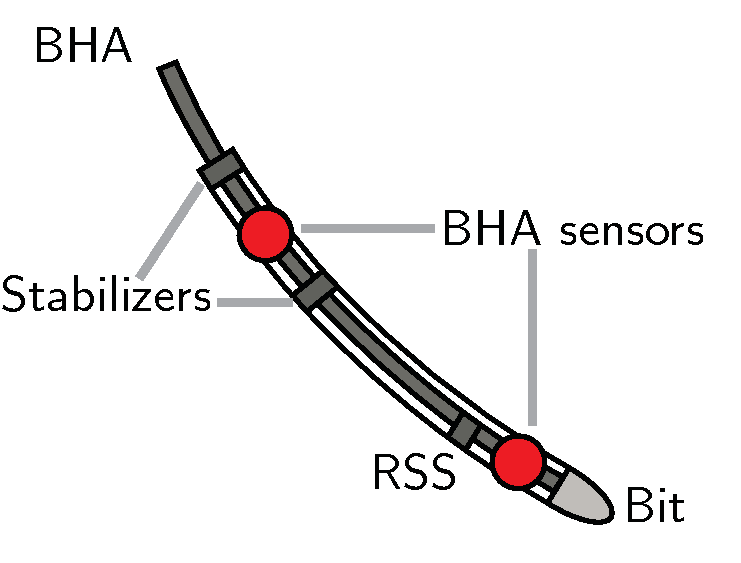
\includegraphics[width=1.1\textwidth]{images/Sensors.pdf}
			\end{figure}
		\end{column}
		\begin{column}{0.45\textwidth}
			\begin{itemize}\setlength\itemsep{1.5em}
				\item Only measurements of the BHA orientation
				\item Equation for sensor location:
				\begin{align*}
				y_{\theta}&=[\theta_0(\xi, s_{m,1}),\; \theta_2(\xi, s_{m,2})]^T \\
				y_{\phi}&=[\phi_0(\xi, s_{m,1}),\; \phi_2(\xi, s_{m,2})]^T
				\end{align*}
				\item Output explicit expressions:
				\begin{align*}
				y_\Theta &= C_\Theta x_\Theta + D_\Theta \Gamma_\Theta + W_y \\
				y_\Phi &= C_\Phi x_\Phi + D_\Phi \frac{\Gamma_\Phi}{\sin \Theta}		
				\end{align*}	
			\end{itemize}
		\end{column}
\end{columns}
\end{frame}

\section{Controller design}

\begin{frame}{Control objectives}
	\begin{itemize}\setlength\itemsep{1.5em}
		\item Track a desired reference trajectory corresponding to a complex borehole geometry
		\item The response of the system should have favorable transient behavior (avoid kinking, rippling and spiraling)
	\end{itemize}
\end{frame}



\begin{frame}{Plant definition}\setlength{\leftmargini}{0pt}
\begin{itemize} 
				\item <1|only@1> [] \begin{figure}[ht]\centering
				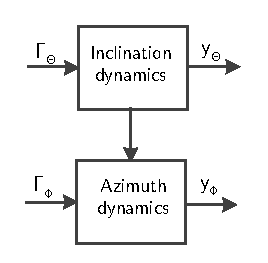
\includegraphics[width=0.7\textwidth]{images/Plant.pdf}
			\end{figure}
			\item <2|only@2> [] \begin{figure}[ht]\centering
				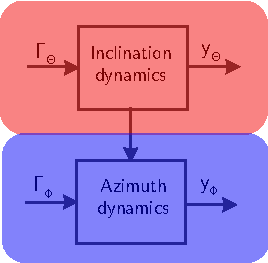
\includegraphics[width=0.7\textwidth]{images/Plant2.pdf}
			\end{figure}
			\item <3|only@3> [] \begin{figure}[ht]\centering
				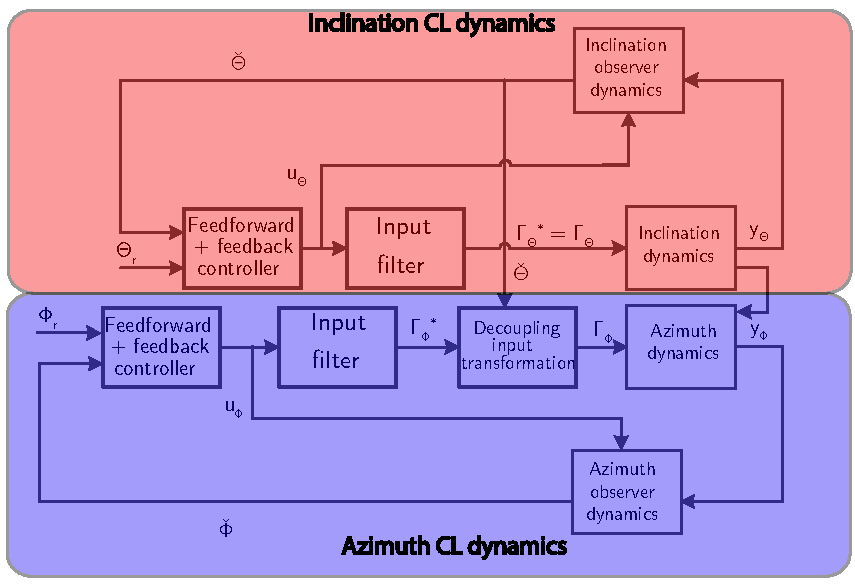
\includegraphics[width=1\textwidth]{images/ControlStrategy0.pdf}
			\end{figure}
\end{itemize}
\end{frame}

\begin{frame}{Control structure}
Input decoupling transformation

\begin{itemize}

	\item <1|only@1> [] \begin{figure}
		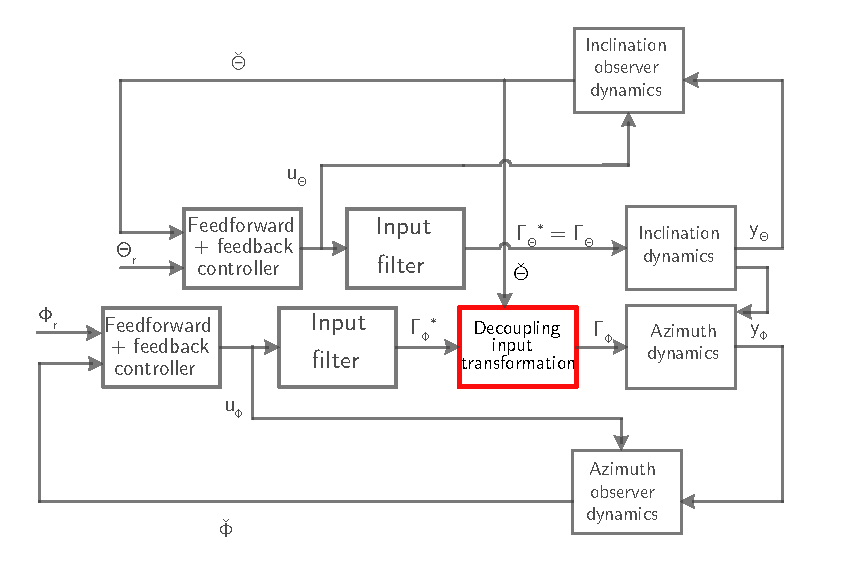
\includegraphics[width=1\textwidth]{images/ControlStrategy1.pdf}
	\end{figure}
	\item <2|only@2> []
	\begin{itemize} 
		\item Coupling terms:
		\footnotesize\begin{equation*}
		\color{gray} \left( {\frac{\chi }{\eta }\frac{{{\mathcal{F}_r}\color{black}\mathlarger{\mathlarger{\boldsymbol{\Theta}}}\color{gray} '\cos \color{black}\mathlarger{\mathlarger{\boldsymbol{\Theta}}}\color{gray} }}{{{{\left( {\sin \color{black}\mathlarger{\mathlarger{\boldsymbol{\Theta}}}\color{gray} } \right)}^2}}} - \frac{{{\mathcal{M}_b}{\mathcal{F}_r} + {\mathcal{M}_r}\left( {\eta \Pi  - {\mathcal{F}_b}} \right)}}{{\eta \Pi \sin \color{black}\mathlarger{\mathlarger{\boldsymbol{\Theta}}}\color{gray} }}} \right){\color{blue}\mathlarger{\mathlarger{\boldsymbol{\Gamma _{\Phi}}}}}\color{gray} - \frac{\chi }{\eta }\frac{{{\mathcal{F}_r}}}{{\sin \color{black}\mathlarger{\mathlarger{\boldsymbol{\Theta}}}\color{gray} }}\color{blue}\mathlarger{\mathlarger{\boldsymbol{\Gamma_{\Phi}'}}}\color{gray}
		\end{equation*}
		
		\item \small Fully decouples system$[$\cite{Monsieurs2015}$]$:
		\begin{equation*}
					\begin{bmatrix}
					\Gamma_{\!\Theta}^* \\ \Gamma_{\!\Phi}^* 	
					\end{bmatrix} :=  \begin{bmatrix} 1 & 0 \\ 0 & \frac{1}{\sin \Theta}\end{bmatrix} \begin{bmatrix}\Gamma_{\!\Theta} \\ \Gamma_{\!\Phi} \end{bmatrix}, \qquad \text{for } \Theta\in (0,\; \pi).
					\nonumber
		\end{equation*}
		\item Problem: no access to $\Theta$
		\begin{equation*}
					\color{gray}\begin{bmatrix}
					\Gamma_{\!\Theta}^* \\ \Gamma_{\!\Phi}^* 	
					\end{bmatrix} :=  \begin{bmatrix} 1 & 0 \\ 0 & \frac{1}{\sin \color{black}\mathlarger{\mathlarger{\boldsymbol{\check{\Theta}}}}}\color{gray}\end{bmatrix} \begin{bmatrix}\Gamma_{\!\Theta} \\ \Gamma_{\!\Phi} \end{bmatrix}, \qquad \text{for } \check{\Theta}\in (0,\; \pi).
					\nonumber
		\end{equation*}
		\item Decouples system providing proper observer
	\end{itemize}
\end{itemize}
\end{frame}
			
\begin{frame}{Control structure}
Input filter
\begin{itemize}
\item <1|only@1> [] \begin{figure}[ht]\centering
	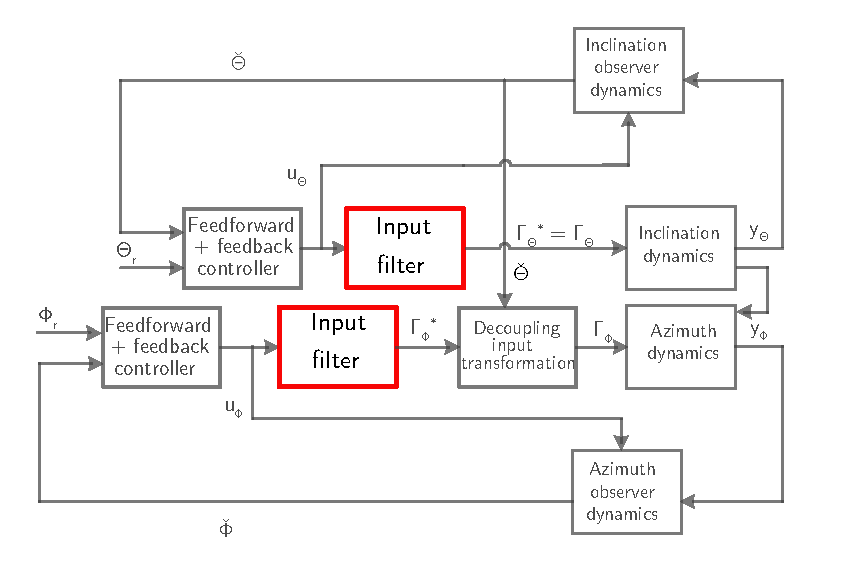
\includegraphics[width=1\textwidth]{images/ControlStrategy2.pdf}
\end{figure}
\item <2|only@2> []\begin{itemize}
 \item Terms with derivative of the input
 \begin{equation*}
			\begin{bmatrix}
			B_{0\Theta} & 0\\
			0 & \boxed{B_{0\Phi}(\Theta,\Theta')}
			\end{bmatrix} 
			\begin{bmatrix}
			\Gamma_\Theta^* \\
			\Gamma_\Phi^*
			\end{bmatrix} +
			\begin{bmatrix}
			B_{1\Theta} & 0\\
			0 & \boxed{B_{1\Phi}(\Theta,\Theta')}
			\end{bmatrix} 
			\begin{bmatrix}
			\Gamma_\Theta^{*'} \\
			\Gamma_\Phi^{*'}
			\end{bmatrix}
\end{equation*}
\item New control input for $i = \Theta, \Phi$
\begin{equation*}
B u_i = B_{0i} \Gamma_i^* + B_{1i} \Gamma_i^{*'}, \qquad B=\begin{bmatrix}
1 & 0 & 0
\end{bmatrix}
\end{equation*}
\item Solve ODE 
\begin{equation*}
\Gamma_i^{*'} = B_{1i}^+ B u_i - B_{1i}^+ B_{0i} \Gamma_i^*
\end{equation*}
\item Problem $\Theta \ne \check{\Theta}$, include $\Gamma_i$ in states
\begin{equation*}
			\begin{bmatrix}
			x_\Theta(\xi) &
			\Gamma_\Theta^{*}(\xi) &
			x_\Phi(\xi) &
			\Gamma_\Phi^{*} (\xi)
			\end{bmatrix}^T
\end{equation*}
\end{itemize}

\end{itemize}
\end{frame}

\begin{frame}{Control structure}
Feedback + feedforward controller
\begin{itemize}
\item <1|only@1> []
\begin{figure}[ht]\centering
	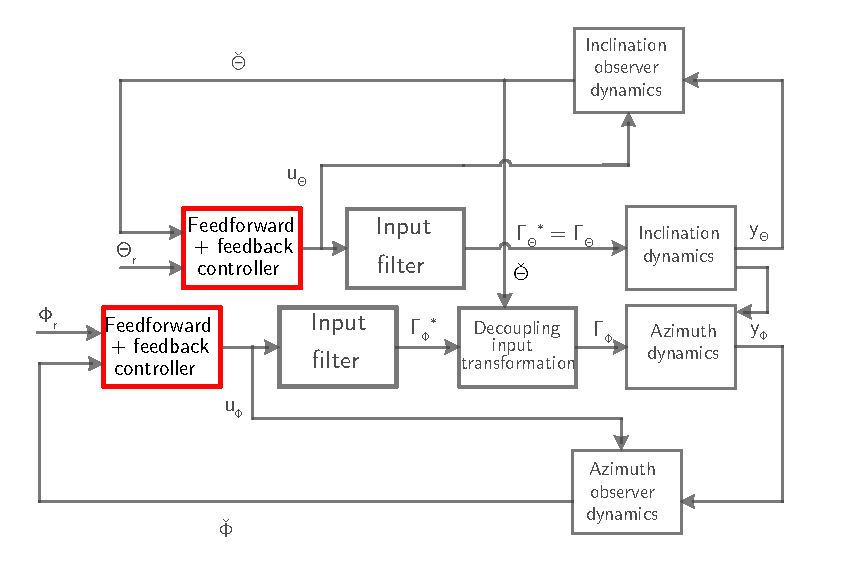
\includegraphics[width=1\textwidth]{images/ControlStrategy3.pdf}
\end{figure}
\item <2|only@2> []
\begin{itemize}
				\item Control input:
				\begin{equation*}
				u_i = v_i + u_{ri}, \text{ for } i = \Theta,\Phi.
				\end{equation*}
				\item Feedforward:
				\begin{equation*}
				u_{ri} = B^T (x'_{ri}(\xi) - A_0 x_{ri}(\xi) - A_1 x_{ri}(\xi_1) - A_2 x_{ri}(\xi_2)).
				\end{equation*} 
				\item Feedback (with $e_i := x_{ri} - x_i$):
				\begin{align*}
				z_{1i}' &= \zeta \begin{bmatrix}
				k_{1i} & 0 & 0
				\end{bmatrix}e_i \\
				z_{2i}' &= -\gamma z_{2i} + \gamma (z_{1i} + K_i e_i)\\
				v_i &= z_{2i}.
				\end{align*}
				\item Integral ($\zeta$) and low-pass filter ($\gamma$) gains fixed
\end{itemize}
\end{itemize}
\end{frame}


\begin{frame}{Control structure}
Observer
\begin{itemize}\setlength{\leftmargini}{0pt}
\item <1|only@1> []
\begin{figure}[ht]\centering
	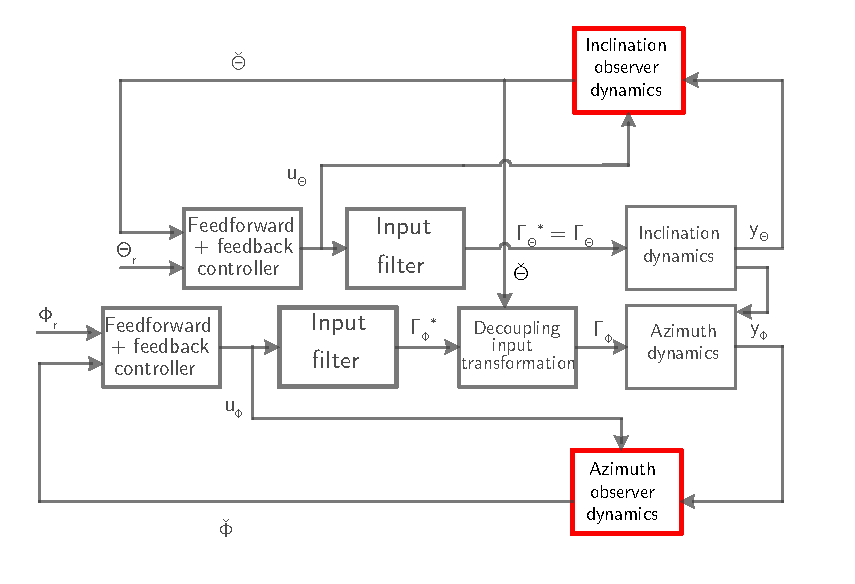
\includegraphics[width=1\textwidth]{images/ControlStrategy4.pdf}
\end{figure}
\item <2|only@2> []
\begin{itemize}\setlength\itemsep{3em}
				\item Only available measurements of the BHA orientation
				\item Model-based observer with output-injection part
				\item Gravity-related terms in the output rejected using integral action:
				\begin{equation*}
				q_i' = \zeta[l_1,l_2](y_i - \check{y}_i), \qquad \text{ for } i=\Theta,\Phi.
				\end{equation*}
\end{itemize}
\item <3|only@3> []
\footnotesize\begin{align*}
		\begin{bmatrix}
		\check{x}_\Theta' \\
		q_\Theta' \\
		\check{x}_\Phi'\\
		q_\Phi'
		\end{bmatrix} &=
		\begin{bmatrix}
		A_0 & 0 & 0 & 0\\
		0 & 0 & 0 & 0\\
		0 & 0 & A_0 & 0 \\
		0 & 0 & 0 & 0 \\
		\end{bmatrix}
		\begin{bmatrix}
		\check{x}_\Theta(\xi) \\
		q_\Theta(\xi) \\
		\check{x}_\Phi(\xi) \\
		q_\Phi (\xi)
		\end{bmatrix} + 
		\begin{bmatrix}
		A_1 & 0 & 0 & 0\\
		0 & 0 & 0 & 0\\
		0 & 0 & A_1 & 0 \\
		0 & 0 & 0 & 0 \\
		\end{bmatrix}
		\begin{bmatrix}
		\check{x}_\Theta(\xi_1) \\
		q_\Theta(\xi_1) \\
		\check{x}_\Phi(\xi_1) \\
		q_\Phi(\xi_1) \\
		\end{bmatrix} \nonumber\\
		\nonumber\\
		&+
		\begin{bmatrix}
		A_2 & 0 & 0 & 0\\
		0 & 0 & 0 & 0\\
		0 & 0 & A_2 & 0 \\
		0 & 0 & 0 & 0 \\
		\end{bmatrix}
		\begin{bmatrix}
		\check{x}_\Theta(\xi_2) \\
		q_\Theta(\xi_2) \\
		\check{x}_\Phi(\xi_2) \\
		q_\Phi(\xi_2) 
		\end{bmatrix} +
		\begin{bmatrix}
		L_\Theta(y_{\Theta} - \check{y}_{\Theta})\\
		\zeta[l_{1\Theta},l_{2\Theta}](y_\Theta - \check{y}_\Theta) \\
		L_{\Phi}(y_{\Phi} - \check{y}_{\Phi}) \\
		\zeta[l_{1\Phi},l_{2{\Phi}}](y_\Phi - \check{y}_\Phi)
		\end{bmatrix} \\
		\\
		&+
		\begin{bmatrix}
		Bq_\Theta \\
		0 \\
		Bq_\Phi \\
		0	
		\end{bmatrix} +
		\begin{bmatrix}
		B(u_{r\Theta} + v_\Theta)\\
		0 \\
		B(u_{r\Phi} + v_\Phi) \\
		0
		\end{bmatrix},\label{eq:Observer}
\end{align*}	
\end{itemize}
\end{frame}


\begin{frame}{Control approach}
	\begin{itemize}\setlength\itemsep{1.5em}
		\item Tune $K_i$ and $L_i$, such that the reference trajectory is the solution of the closed-loop dynamics
		\item Tracking error dynamics and observer error dynamics:
		\begin{equation*}
			e_i := x_{ri} - x{i}, \qquad \delta_i := x_i - \hat{x}_i, \text{ for } i=\Theta,\Phi.
		\end{equation*}
		\item \textbf{Linearize system around}:
		\begin{equation*}
			e_i = 0, \qquad \delta_i = 0.
		\end{equation*}
		\item Linearized closed-loop system: \textbf{$\xi$-dependent}
	\end{itemize}
\end{frame}



\begin{frame}{Controller synthesis}
\vspace{-1cm}
Analysis of the structure of closed-loop matrices:
\\
\vspace{0.5cm}\begin{itemize}\setlength\itemsep{3.5em}
	\item $K_i$ and $L_i$ separation principle for both $\Theta$ and $\Phi$
	\item $\xi$-dependent terms present in coupling terms
	\item Isolated dynamics of $e_i$ and $\delta_i$ are $\xi$-independent (bounded)
\end{itemize}
\end{frame}

\begin{frame}{Controller synthesis}
\begin{itemize}\setlength\itemsep{1.5em}
	\item Synthesize $K_i$ and $L_i$ for isolated systems
	\item Favorable transients, with proper order of convergence
	\item Due to infinite number of poles in delay systems, optimize location of right-most pole over $K_i$ and $L_i$
\end{itemize}
	\begin{figure}[ht]\centering
		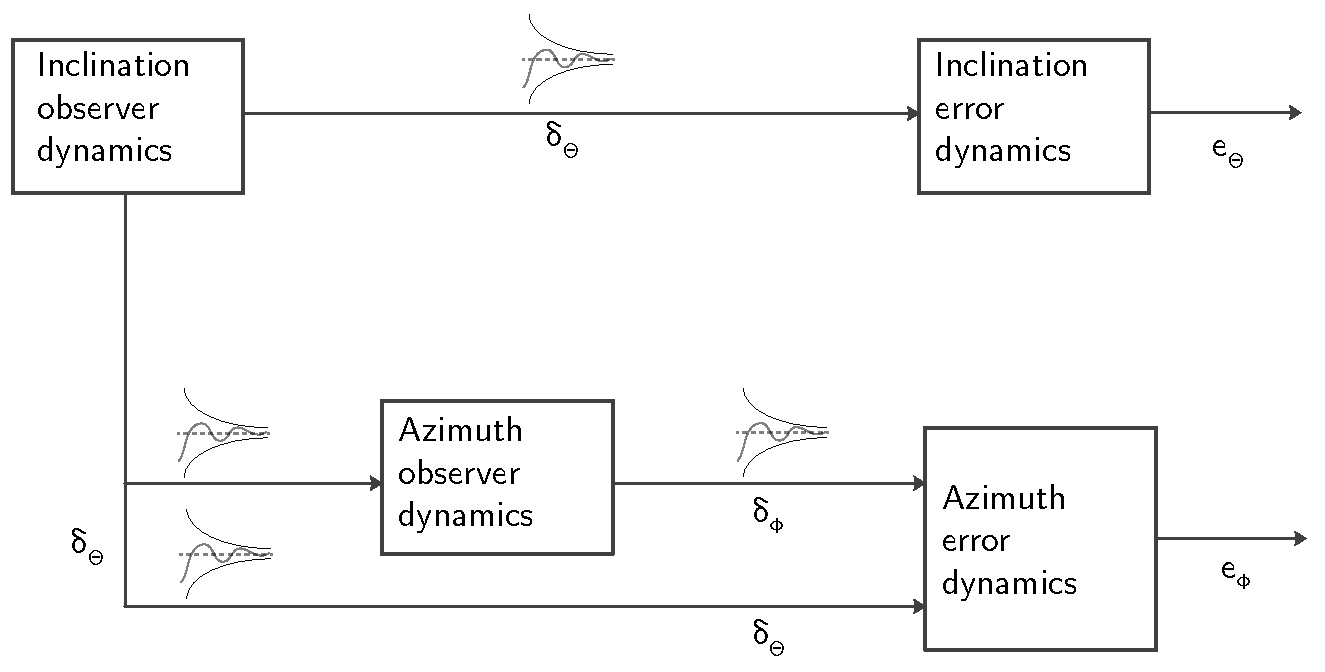
\includegraphics[width=0.7\textwidth]{images/ISS.pdf}
	\end{figure}
\end{frame}


\section{Simulation results}

\begin{frame}{Reference trajectory}
\begin{figure}[t]
	\centering
	\begin{minipage}[b]{0.5\textwidth}
		\centering
		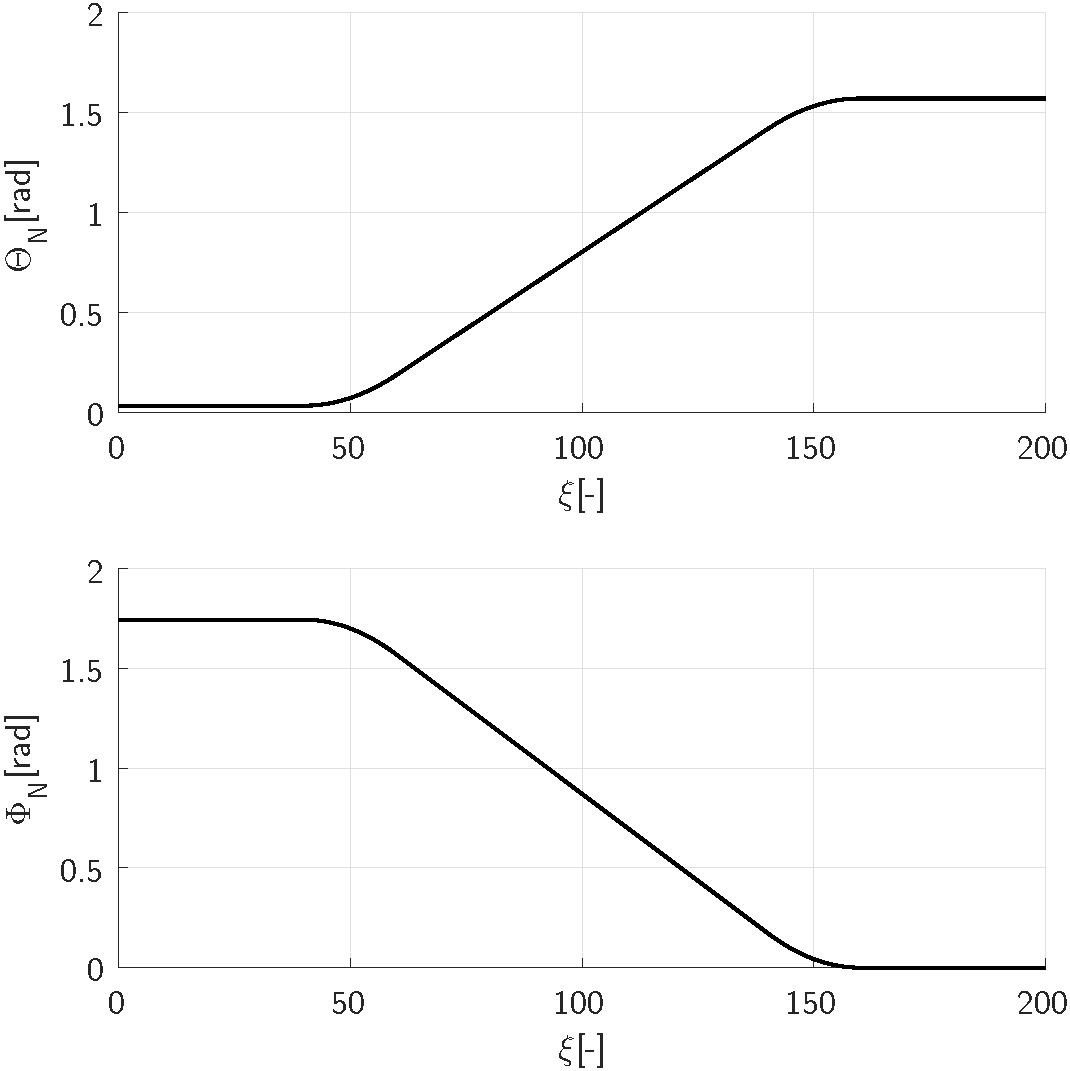
\includegraphics[height=2.3in]{ReferenceTrajectoryThetaPhi.pdf}
		\label{fig:ReferenceTrajectoryThetaPhi} 
	\end{minipage}
	\begin{minipage}[b]{0.45\textwidth}
		\centering
		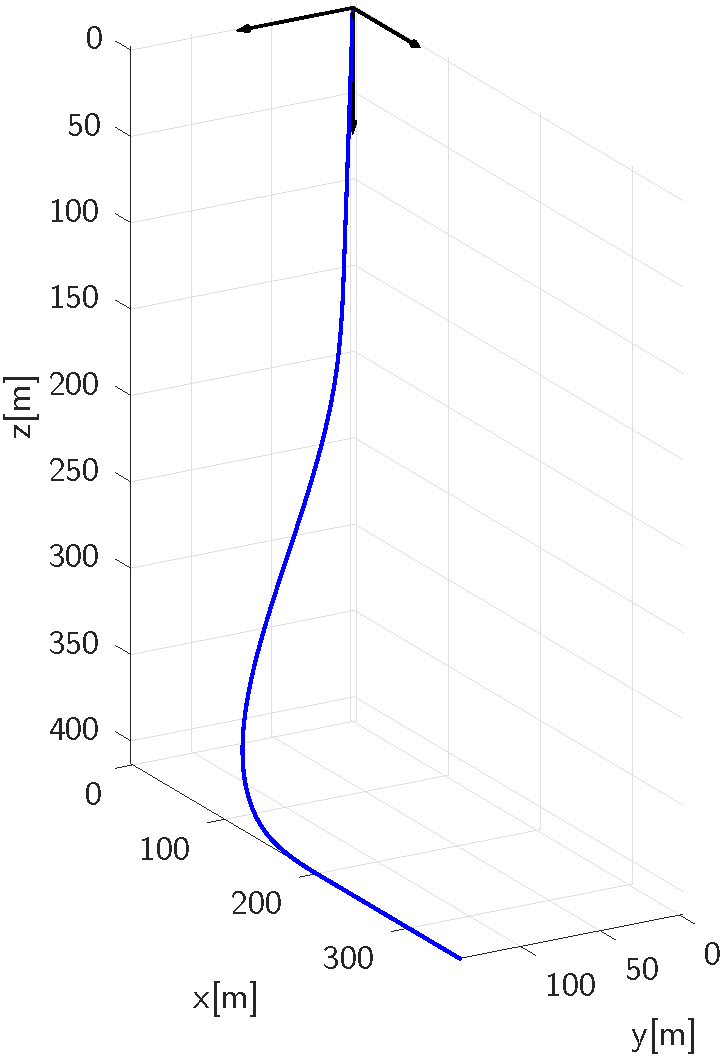
\includegraphics[height=2.3in]{ReferenceTrajectory.pdf}
		\label{fig:ReferenceTrajectoryV} 
	\end{minipage}
\end{figure}
\end{frame}

\begin{frame}{"Time" domain simulation}
\begin{figure}[H]
		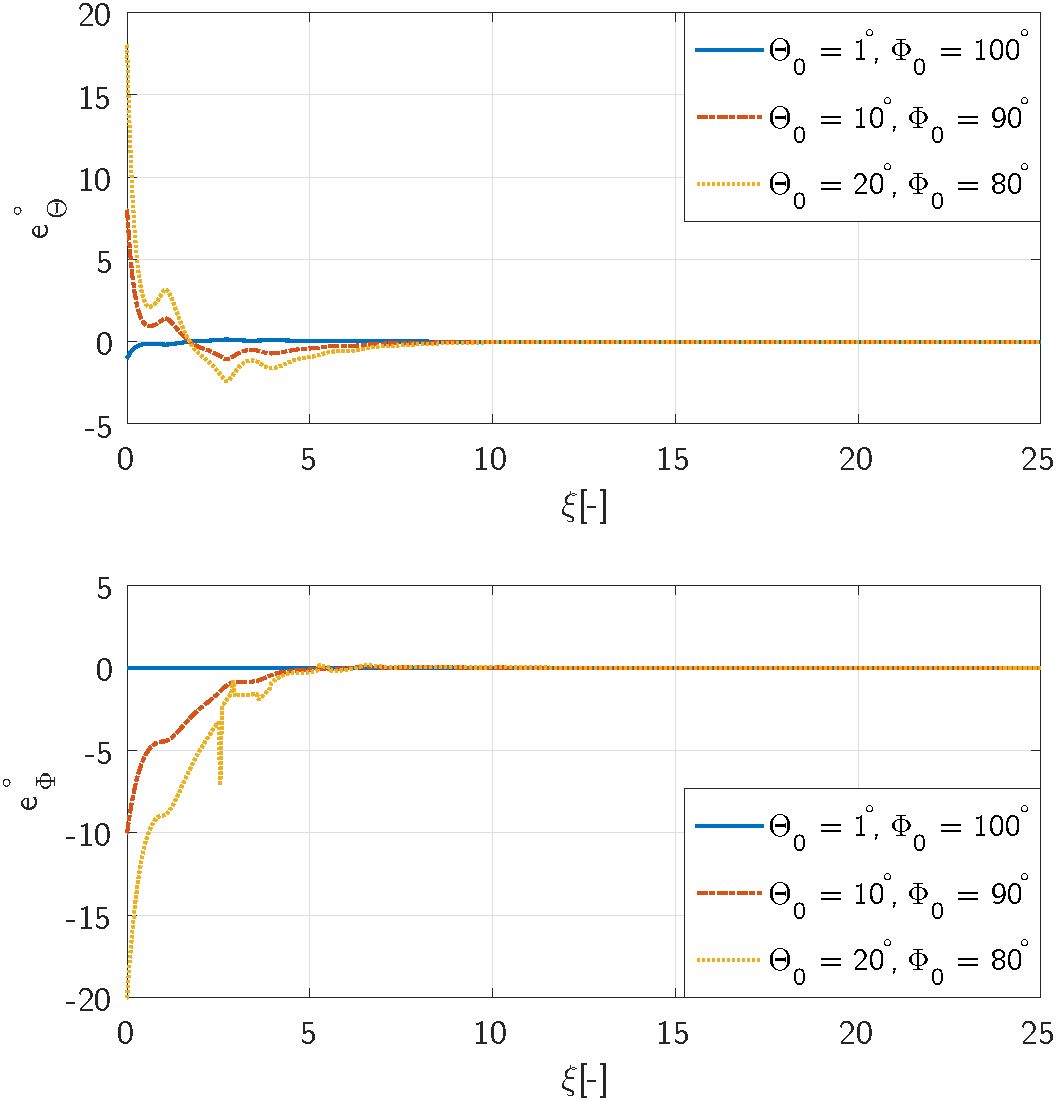
\includegraphics[height=3.25in]{ErrorsNeutral.pdf}
\end{figure}
\end{frame}


\begin{frame}{Robust stability analysis, uncertainty in $\Pi$}
	Closed-loop right-most pole of the system for $\Pi \in [0.5\bar{\Pi},1.5\bar{\Pi}]$
		\begin{columns}[T]
			\hspace{0.5cm}\begin{column}{0.45\textwidth}
				\begin{figure}[ht]
					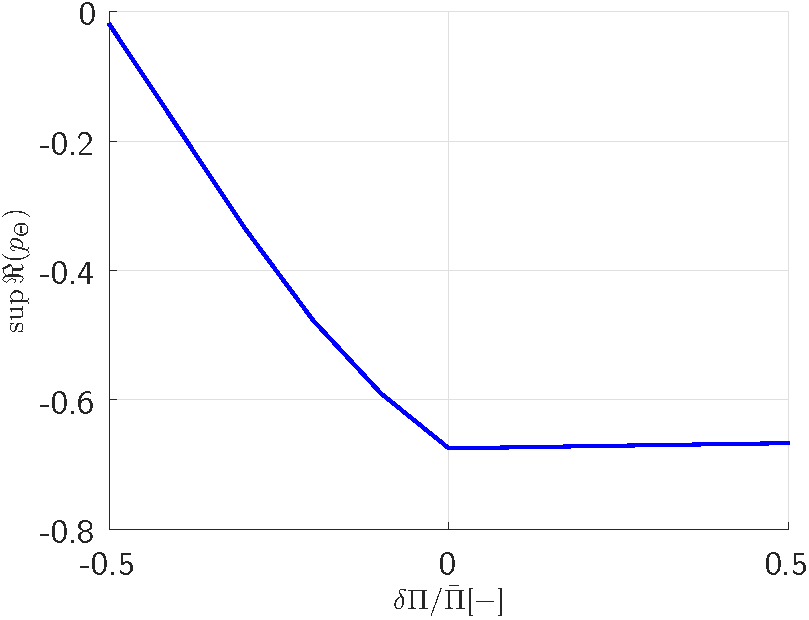
\includegraphics[width=1\textwidth]{images/RobustTestNominalInclination.pdf}
				\end{figure}
				\centering\LARGE Inclination
			\end{column}
			\hspace{0.5cm}\begin{column}{0.45\textwidth}
				\begin{figure}[ht]
					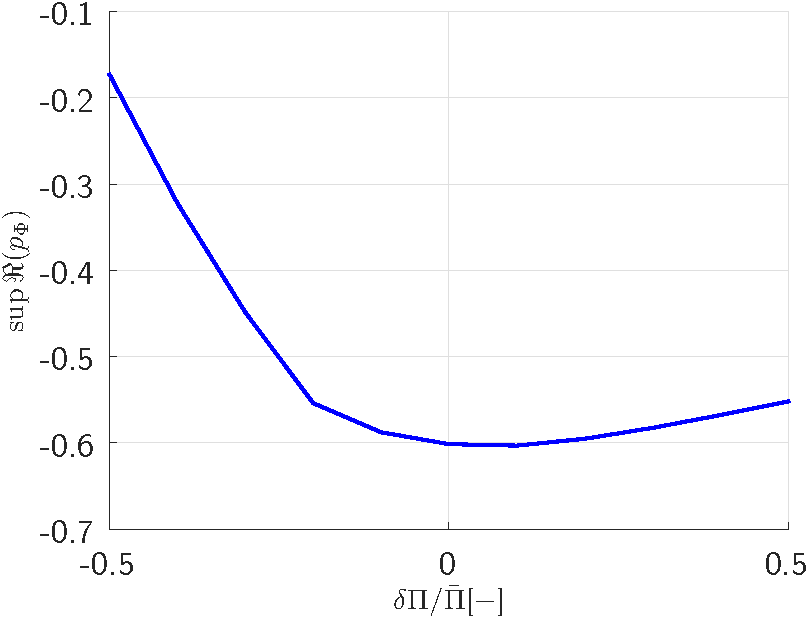
\includegraphics[width=1\textwidth]{images/RobustTestNominalAzimuth.pdf}
				\end{figure}	
			\centering	\LARGE Azimuth		
			\end{column}
		\end{columns}	
\end{frame}


\begin{frame}{"Time" domain simulation, $\Pi = 0.5 \bar{\Pi}$}
		\begin{figure}[ht]\centering
			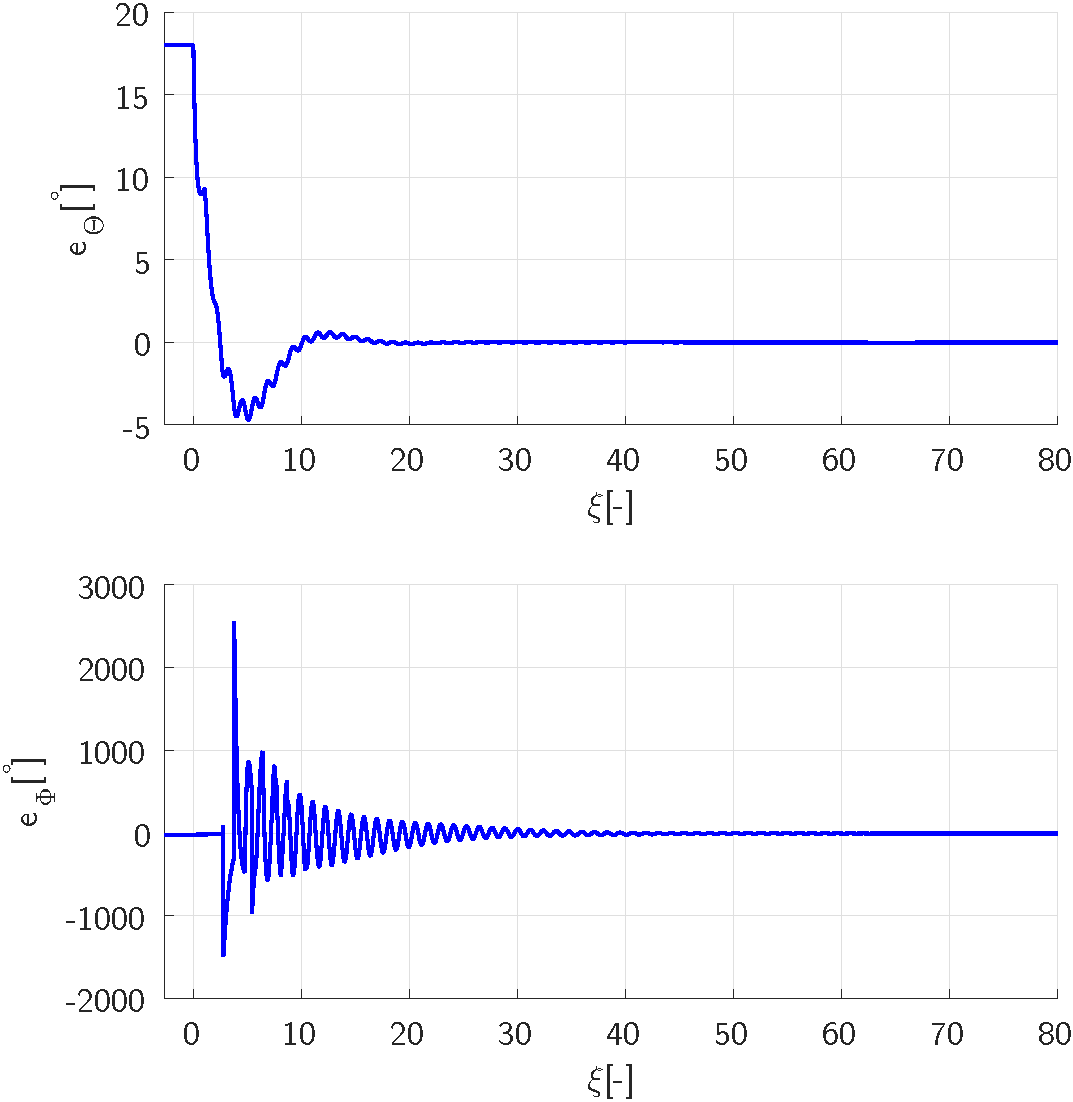
\includegraphics[width=0.7\textwidth]{images/ErrorsNeutralNominal.pdf}
		\end{figure}
\end{frame}

\begin{frame}{Robust controller synthesis}
	\begin{itemize}\setlength\itemsep{3.5em}
		\item Optimize location of right-most pole of closed-loop system for a grid of values of $\Pi \in [0.5 \bar{\Pi}, 1.5 \bar{\Pi}]$
		\item Interval of $\Pi$
		\begin{equation}
		\delta \Pi_i = -\delta \Pi_{max} + \frac{i - 1}{m - 1} 2\delta \Pi_{max}, \qquad \text{ for } i\in \{1,2,...,m\}. \nonumber 
		\end{equation} (this case m = 7)
		\begin{equation*}
		\Pi = \bar{\Pi} + \delta \Pi
		\end{equation*}
	\end{itemize}
\end{frame}

\begin{frame}{Robustness comparison}
	Closed-loop right-most pole of the system for $\Pi \in [0.5\bar{\Pi},1.5\bar{\Pi}]$
		\begin{columns}[T]
			\hspace{0.5cm}\begin{column}{0.44\textwidth}
				\begin{figure}[ht]\centering
					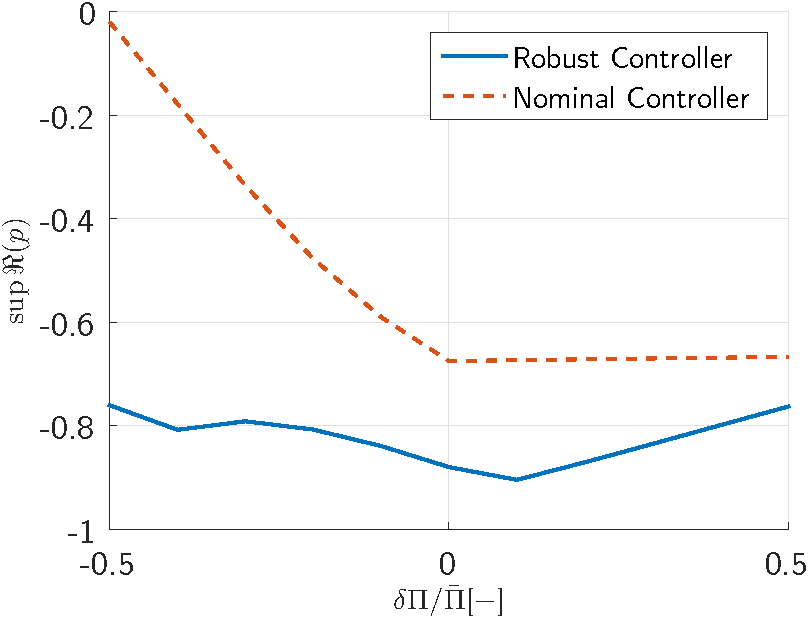
\includegraphics[width=1\textwidth]{images/RobustTestComparisonInclination.pdf}
				\end{figure}
				\centering\LARGE Inclination
			\end{column}
			\hspace{0.5cm}\begin{column}{0.44\textwidth}
				\begin{figure}[ht]\centering
					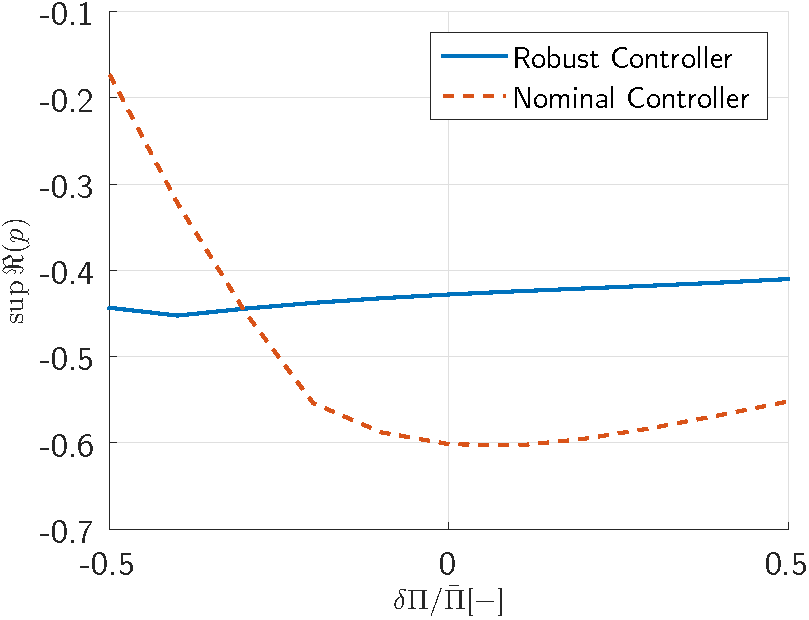
\includegraphics[width=1\textwidth]{images/RobustTestComparisonAzimuth.pdf}
				\end{figure}	
			\centering	\LARGE Azimuth		
			\end{column}
		\end{columns}	
\end{frame}


\begin{frame}{"Time" domain simulation for $\Pi = 0.5\bar{\Pi}$}
		\begin{figure}[ht]\centering
			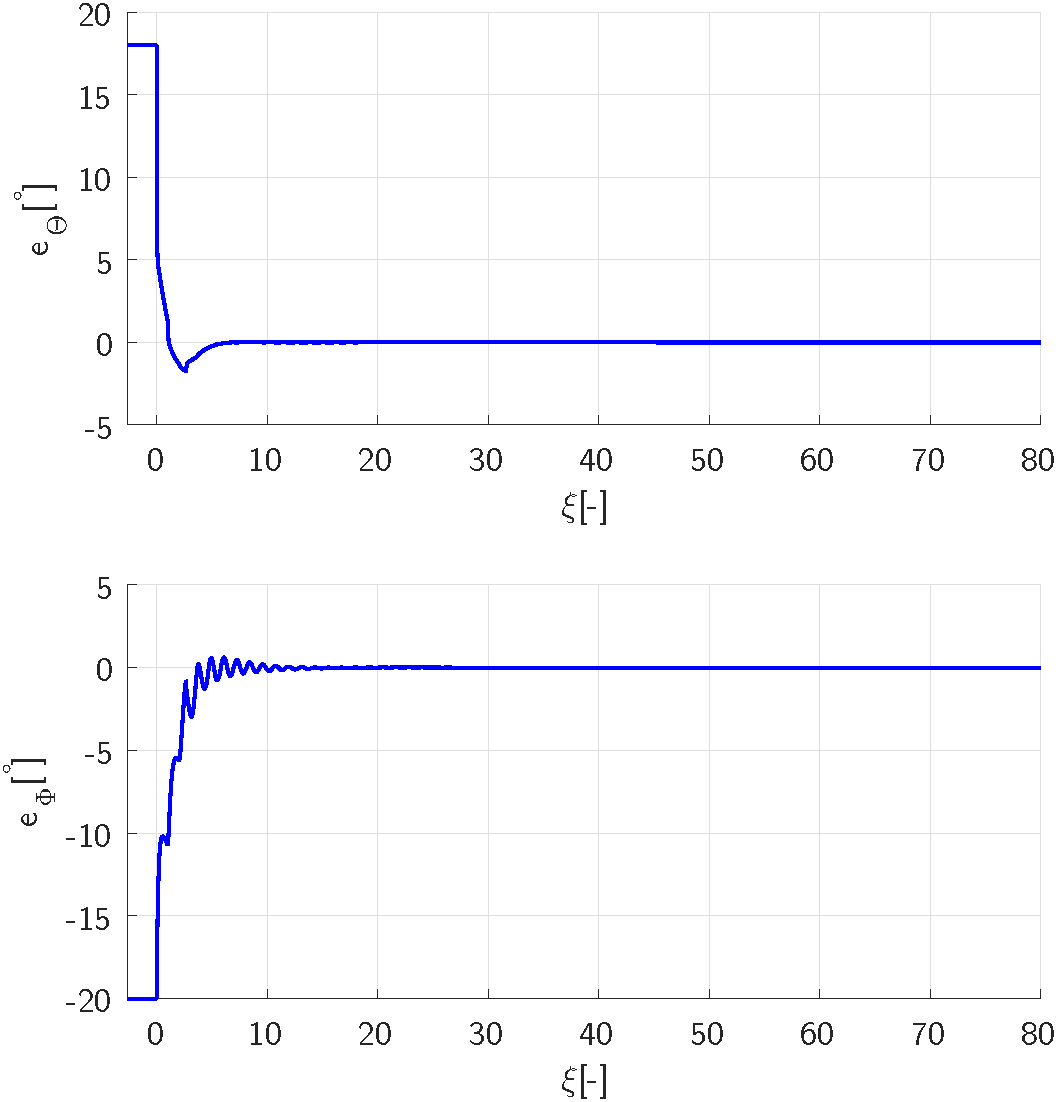
\includegraphics[width=0.7\textwidth]{images/ErrorsNeutralRobust.pdf}
		\end{figure}
\end{frame}

\section{Conclusions and recommendations}


\begin{frame}{Conclusions}
	\begin{itemize}\setlength\itemsep{3em}
		\item A controller that only relies on local measurements of the BHA orientation was developed by means of an observer
		\item The strategy yields robustness against uncertainty in the active weight on bit $\Pi$
		\item Negative effects are greatly reduced even under extreme conditions of low weight on bit
	\end{itemize}
\end{frame}

\begin{frame}{Recommendations}
	\begin{itemize}\setlength\itemsep{3em}
		\item Extend current design to non-neutral bit walk tendency
		\item Study alternative angle parameterization
		\item Analyze use of the developed strategy for models with non-linear effects (bit-tilt saturation, non-ideal stabilizer contact)
	\end{itemize}
\end{frame}

\begin{frame}
Thank you for your attention. Any questions?
\end{frame}


\end{document}
